\subsection{Overfitting and Convergence}
\label{parametersDerivation}
Various methods of derivation of the knowledge-based potentials usually produce results biased towards the training data set. 
Typically, such algorithms maximize the predictive accuracy of the corresponding potential on a set of training data, 
which does not mean that the same potential will perform equally well on a new set of data. 
Indeed, fitting the potential to the training data set also fits the noise in the data. Thus, very often a knowledge-based potential memorizes noisy features 
of the training data instead of deducing general predictive concepts from it.
This phenomenon is usually referred 
to as {\em overfitting} \cite{Dietterich1995}.
%
A clear indication of an "overfitted" potential can be, for example, the need for post-smoothing techniques applied to the initial knowledge-based potential, 
as in \cite{Huang2008, mitchell1999bleep}.
"Overfitting" is clearly not desirable. In order to avoid it, many optimization techniques (regularization, cross-validation, etc.) 
have been successfully proposed to penalize the initial objective function with various additional terms \cite{Arlot2010, Kearns1997}. 
These  terms serve to achieve a better predictive accuracy on the off-training data based on the predictions of the training data.

To avoid overfitting, we used two techniques -- {\em regularization} and {\em cross-validation}. 
Regularization penalizes the initial objective function with various additional terms \cite{Arlot2010, Kearns1997}. 
We introduced two regularization parameters, $\sigma$ for the width of the Gaussian distribution of distances in Eq. \ref{eq:number_density}, and  $C$ for the 
hinge loss function in Eq. \ref{eq:svmSoftMargin}. 
%
%
To find the best values of these parameters we used the following cross-validation procedure.
First, we divided the training set into two parts, consisting of 650 complexes (temporary test set) and 200 complexes (temporary training set). 
Then, for each value of $\sigma$ and $C$, we obtained the scoring potentials using the temporary training set and verified it on the temporary test set.
Finally, we chose those values of $\sigma$ and $C$ that correspond to the maximum number of guessed structures in the temporary test set. 
We define the structure as guessed if its native complex has the score better than all of its decoys.	
Figure \ref{fig:crossVal} shows 
the predictive performance of the scoring potential on the two sets as a function of $\sigma$ and $C$. 
Obviously, the maximum predictive performance on the training set is achieved at the highest values of $C$. 
However, the validation on the test set highlights 
the best choice of values of $C$ and $\sigma$.
%
These values are $C=10^6\dots10^7$ and $\sigma=0.4$ \AA~ (Fig. \ref{fig:crossVal}B).

Figure \ref{fig:convergence} shows the convergence of the success rate on the training set with the number of iterations of the training BSMO algorithm.
The success rate was measured as the number of guessed structures divided by the total number of protein-protein complexes. 
We can see a fast convergence of the method. In principle, a hundred optimization steps is sufficient to obtain the final result. 
We have also observed that  increasing  the regularization parameter $C$ leads
to the slower convergence and vice versa. 
We should note that thanks to the convexity of our optimization problem, its solution is unique and does not depend on the starting point and the optimization method used.


\begin{figure}[H]
\begin{center}
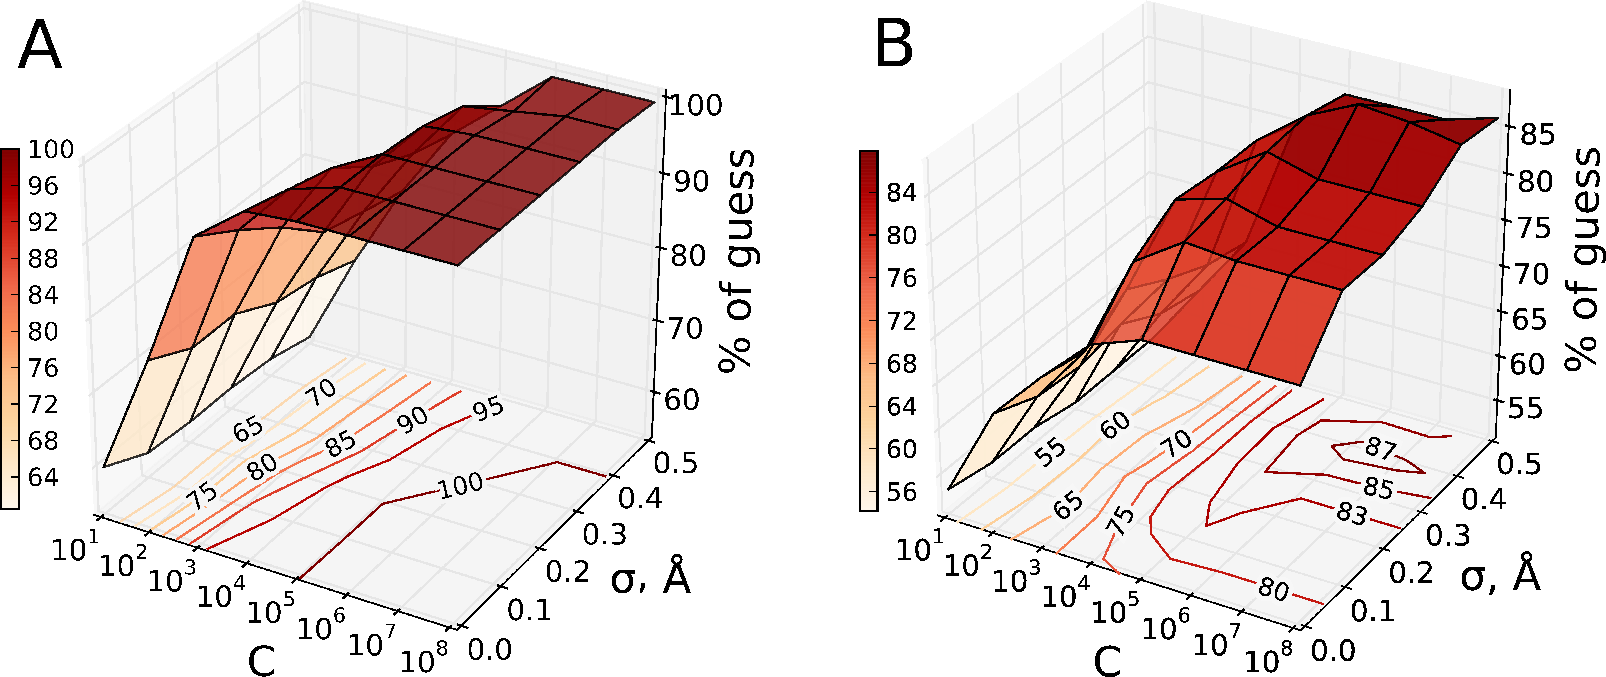
\includegraphics[scale=0.4]{Scoring/Fig/2plots_final}
\caption[Predictive performance of the scoring potential as a function of the smoothing parameter $\sigma$ and the regularization parameter $C$]{
Predictive performance of the scoring potential as a function of the smoothing parameter $\sigma$ and the regularization parameter $C$. 
A) Performance obtained if the scoring functions are trained on the whole database and verified on the same database. 
B) Performance obtained if the scoring functions are trained on 200 protein complexes and verified on the other 650 complexes from the training database.
Here the best performance is obtained with $\sigma=0.4$ \AA~ and $C=10^6\dots10^7$.
}
\label{fig:crossVal} 
\end{center}
\end{figure}

\begin{figure}[H]
\begin{center}
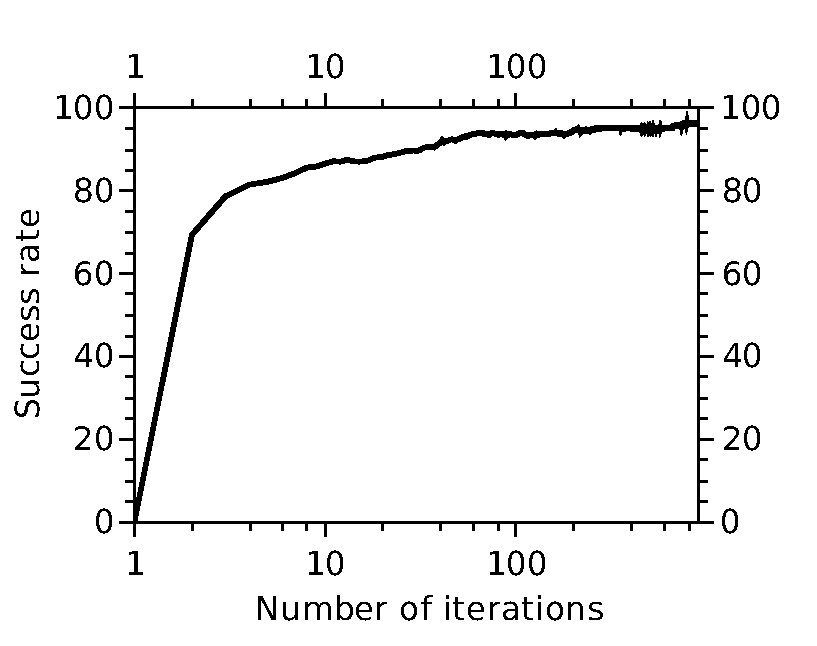
\includegraphics[scale=0.8]{Scoring/Fig/SuccessRateVsNIter}
\caption[Performance rate of the scoring potentials on the training set versus the number of iterations of the BSMO algorithm]{
Performance rate of the scoring potentials on the training set versus the number of iterations of the BSMO algorithm. The scoring potentials were obtained using the Legendre basis and the whole
training set, without excluding any homologous proteins. Parameters $\sigma$ and $C$ were set to the optimal values of $\sigma=0.4$ \AA~ and $C=10^5$.
}
\label{fig:convergence} 
\end{center}
\end{figure}


\subsection{Extracted Potentials}
Our method can in principle use any type of orthogonal polynomials to decompose the structural statistics and reconstruct the potentials. 
However, since rectangular functions are the most widely used to collect  statistics, we employed this basis as a reference. 
Then, we also used the Legendre basis, orthogonal on the interval [0;10]. We chose this basis because of its simplicity, in particular because 
the weight function for this basis does not depend on the distance.
%

From now on, we call the obtained scoring potentials the Convex Protein Protein (ConvexPP) potentials. 
Figure \ref{fig:potentials} shows typical scoring potentials derived using two different orthogonal bases. 
%
Obtained potentials are smooth by construction, thanks to the smooth Gaussian kernel in Eq. \ref{eq:scoring_2}.
%
According to the plot, the shape of the potentials does not depend on the basis set that was
used to derive it. This is the consequence of the global convergence of the optimization problem (see lemma \ref{lemma2}).
We can also see that the obtained potentials tend to zero as the interaction distance increases. On the other hand, all the potentials approach zero at short distances. 
This is due to the absence of statistics for the native structures at short distances and the result of the $ \mathbf{w}\cdot\mathbf{w}$ term in optimization problem \ref{eq:svmSoftMargin}. 
We discuss this behaviour in more detail below.

%
Due to the Gaussian smoothing of statistics, 
%with variance $\sigma$, 
it is sufficient to use the expansion order of $P = r_{max}/{\sigma}$. 
For $\sigma=0.4$ \AA~ and $ r_{max}=10$ \AA , the estimate on the number of basis functions is $P=25$. 
However, due to the adjustment of $\sigma$ with the cross-validation procedure, in our experiments we used a larger expansion order,  $P=40$.
%, that exceeds the lower estimate. 
%After the parameter $\sigma$ is determined, one can lower the degree of the polynomial expansion to 25.
Figure \ref{fig:potentialsDec} demonstrates how the resulting potentials depend on the expansion order. We should note that the decompositions of orders above 25 are almost indistinguishable and thus are not shown. 
Indeed,
increasing the order of the polynomial $P$ decreases the distance between two consecutive zeros in the polynomial basis. Therefore, at a constant value of $\sigma$, the integral in Eq. (\ref{eq:projection})
tends to zero with the growth of the value of $P$ due to the oscillatory behaviour of the basis polynomials. Such behaviour of the integral confines all the useful  information 
about the distributions and the scoring potentials in the first few coefficients of the polynomial decomposition. The number of these coefficients depends solely on the value of $\sigma$ 
and does not change with the training set
or the value of  parameter $C$.

\begin{figure}[H]
\begin{center}
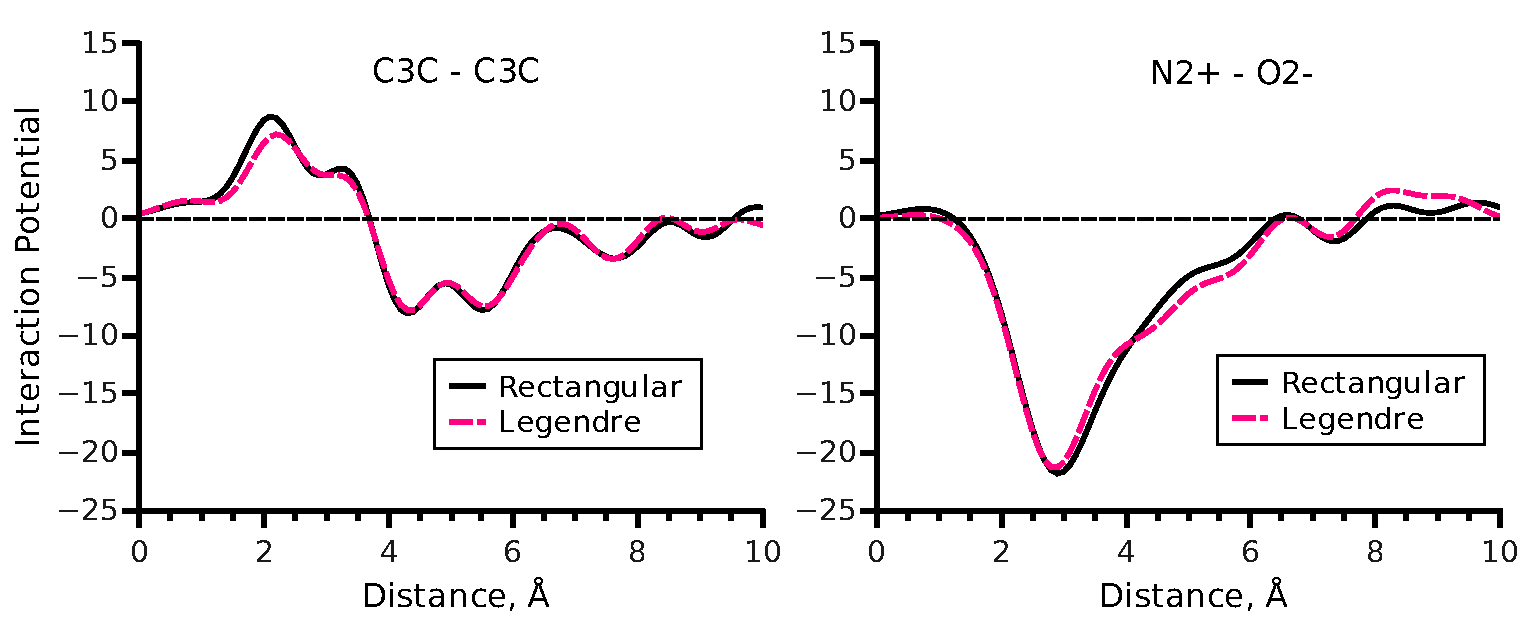
\includegraphics[width=0.75\textwidth]{Scoring/Fig/2functions}
\caption[The scoring potentials trained in two different polynomial bases]{The scoring potentials trained in two different polynomial bases. Dashed lines correspond to the scoring potentials that were obtained using the Legendre basis functions. 
Solid lines correspond to the potentials that were obtained using the rectangular basis functions. 
%The values of both types of potentials on the grid were obtained using Eq. (\ref{eq:scoring_2}).}
Left: Potential between aliphatic carbons bonded to carbons or hydrogens only.
Right: Potential between a guanidine nitrogen with two hydrogens and an oxygen in carboxyl groups.
}
\label{fig:potentials} 
\end{center}
\end{figure}

\begin{figure}[H]
\begin{center}
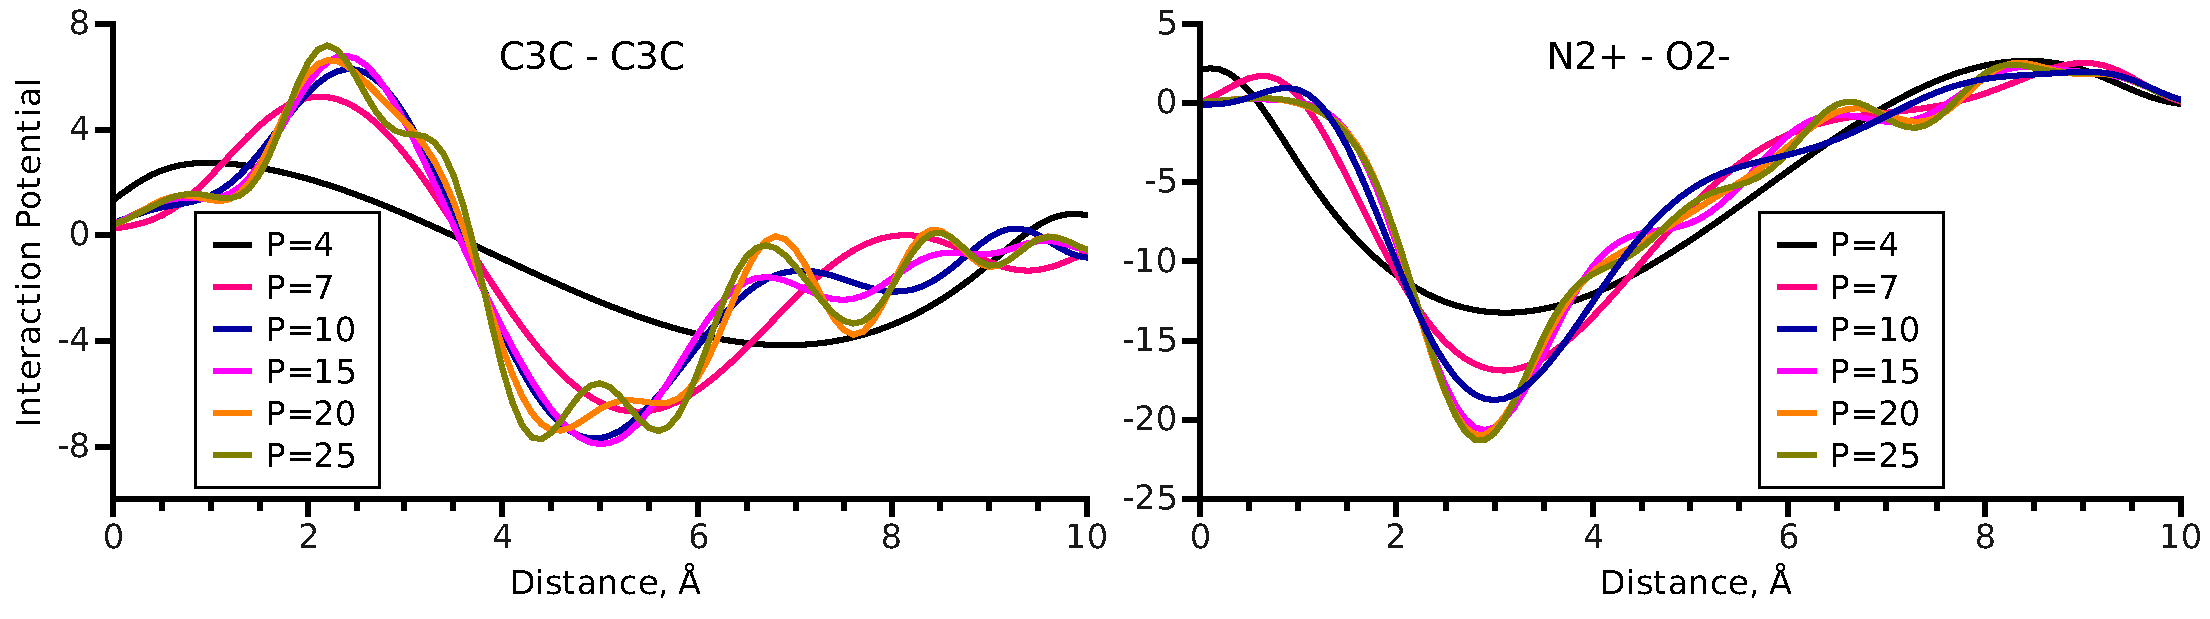
\includegraphics[width=0.85\textwidth]{Scoring/Fig/adaptivity_01}
\caption[Dependence of the extracted scoring potentials on the order of the decomposition in the Legendre basis]{
Dependence of the extracted scoring potentials on the order of the decomposition in the Legendre basis. After order $P=25$, the potentials are indistinguishable from each other and thus not shown for clarity.
%
Left: Potential between aliphatic carbons bonded to carbons or hydrogens only.
Right: Potential between a guanidine nitrogen with two hydrogens and an oxygen in carboxyl groups.
}
\label{fig:potentialsDec} 
\end{center}
\end{figure}


\subsection{Protein-Protein docking benchmark version 3.0}
First we tested the ConvexPP scoring function on the protein-protein docking benchmark version 3.0. It consists of 124 crystallographic structures of protein-protein complexes 
from PDB database \cite{hwang2008protein}. They are divided into three groups: rigid,
medium and difficult cases. The division criteria is the scale of conformational changes of the proteins upon binding: from minor changes in rigid cases to major in difficult. 
The nonredundancy of the benchmark was set at the level of 
family-family pairs. That means that if a complex in Benchmark v3.0 is formed of the protein of family A and another one of family B,
then there are no more family A - family B complex in the benchmark. The assignment of a protein to a family was taken according to SCOP database \cite{murzin1995scop}.

The decoys for scoring were generated using ZDOCK3.0 \cite{pierce2011accelerating} with the sampling step equal to 6 degrees (we call this set of docking position \emph{ZDOCK benchmark} below).
They were downloaded from the ZLAB website \cite{ZDOCKDecoysLink}.
The docking program ZDOCK3.0 generates the rigid-body protein-protein docking predictions with the corresponding scores.
Scoring function used in this program includes shape complementarity, statistical pair potentials and electrostatics. 
To compare our scoring function to the well established one downloaded the decoy set reranked by ZRANK \cite{pierce2007zrank}. 
It is the program for reranking the ZDOCK3.0 predictions. 
In addition to the factors used in ZDOCK3.0, it computes detailed electrostatics, estimates desolvation and uses additional Van-der-Waals potential to re-score the decoys. 

The benchmark 3.0 has several complexes homologous to certain protein complexes in the training set. Therefore, to see the effect of training set and test set similarity
we trained our potential both excluding homologs from the training set and leaving it unchanged. 
Table \ref{ZDockTable} shows results of ZDOCK3.0, ZRANK and our scoring functions on the ZDOCK benchmark.

\newpage

\begin{longtable}{c c c c c|c c c c|c c c c}
& 
\multicolumn{4}{c}{ZDock} &
\multicolumn{4}{c}{ZRank} &
\multicolumn{4}{c}{ConvexPP} \\
\hline
\begin{sideways}{Complex}\end{sideways}&\begin{sideways}{Rank}\end{sideways}&\begin{sideways}$\mathrm{L_{rmsd}}$\end{sideways}&\begin{sideways}$\mathrm{I_{rmsd}}$\end{sideways}&\begin{sideways}$\mathrm{F_{nat}}$\end{sideways}&\begin{sideways}{Rank}\end{sideways}&\begin{sideways}$\mathrm{L_{rmsd}}$\end{sideways}&\begin{sideways}$\mathrm{I_{rmsd}}$\end{sideways}&\begin{sideways}$\mathrm{F_{nat}}$\end{sideways}&\begin{sideways}{Rank}\end{sideways}&\begin{sideways}$\mathrm{L_{rmsd}}$\end{sideways}&\begin{sideways}$\mathrm{I_{rmsd}}$\end{sideways}&\begin{sideways}$\mathrm{F_{nat}}$\end{sideways}\\ 
 \hline
\multicolumn{13}{c}{Rigid-Body}\\
{\tiny 1AHW} &{\tiny 54}&{\tiny 8.30}&{\tiny 1.58}&{\tiny 0.60} &{\tiny 175}&{\tiny 2.68}&{\tiny 1.26}&{\tiny 0.72} &{\tiny 547}&{\tiny 2.14}&{\tiny 0.91}&{\tiny 0.79}\\ 
 {\tiny 1BVK} &{\tiny -}&{\tiny -}&{\tiny -}&{\tiny -} &{\tiny -}&{\tiny -}&{\tiny -}&{\tiny -} &{\tiny -}&{\tiny -}&{\tiny -}&{\tiny -}\\ 
 {\tiny 1DQJ} &{\tiny -}&{\tiny -}&{\tiny -}&{\tiny -} &{\tiny -}&{\tiny -}&{\tiny -}&{\tiny -} &{\tiny -}&{\tiny -}&{\tiny -}&{\tiny -}\\ 
 {\tiny 1E6J} &{\tiny 1}&{\tiny 3.80}&{\tiny 1.59}&{\tiny 0.64} &{\tiny 12}&{\tiny 6.06}&{\tiny 2.35}&{\tiny 0.40} &{\tiny 35}&{\tiny 4.21}&{\tiny 2.26}&{\tiny 0.48}\\ 
 {\tiny 1JPS} &{\tiny 1}&{\tiny 3.90}&{\tiny 1.04}&{\tiny 0.70} &{\tiny 254}&{\tiny 4.32}&{\tiny 1.26}&{\tiny 0.65} &{\tiny 62}&{\tiny 4.14}&{\tiny 1.11}&{\tiny 0.78}\\ 
 {\tiny 1MLC} &{\tiny 5}&{\tiny 4.61}&{\tiny 1.14}&{\tiny 0.36} &{\tiny 54}&{\tiny 4.61}&{\tiny 1.14}&{\tiny 0.36} &{\tiny 5}&{\tiny 4.70}&{\tiny 1.12}&{\tiny 0.39}\\ 
 {\tiny 1VFB} &{\tiny 997}&{\tiny 10.89}&{\tiny 2.48}&{\tiny 0.30} &{\tiny 798}&{\tiny 0.89}&{\tiny 2.48}&{\tiny 0.30} &{\tiny 1239}&{\tiny 10.89}&{\tiny 2.48}&{\tiny 0.30}\\ 
 {\tiny 1WEJ} &{\tiny 2}&{\tiny 2.44}&{\tiny 0.79}&{\tiny 0.91} &{\tiny 41}&{\tiny 2.44}&{\tiny 0.79}&{\tiny 0.91} &{\tiny 1}&{\tiny 4.13}&{\tiny 1.30}&{\tiny 0.75}\\ 
 {\tiny 2FD6} &{\tiny 15}&{\tiny 18.67}&{\tiny 2.42}&{\tiny 0.73} &{\tiny 9}&{\tiny 9.76}&{\tiny 2.42}&{\tiny 0.80} &{\tiny 8}&{\tiny 15.65}&{\tiny 2.16}&{\tiny 0.80}\\ 
 {\tiny 2I25} &{\tiny 1534}&{\tiny 7.92}&{\tiny 2.21}&{\tiny 0.36} &{\tiny 1}&{\tiny 4.45}&{\tiny 1.87}&{\tiny 0.33} &{\tiny 83}&{\tiny 4.45}&{\tiny 1.87}&{\tiny 0.33}\\ 
 {\tiny 2VIS} &{\tiny 8}&{\tiny 27.81}&{\tiny 2.02}&{\tiny 0.63} &{\tiny 150}&{\tiny 6.31}&{\tiny 2.18}&{\tiny 0.57} &{\tiny 617}&{\tiny 23.89}&{\tiny 2.37}&{\tiny 0.43}\\ 
 {\tiny 1BJ1} &{\tiny 19}&{\tiny 6.29}&{\tiny 1.19}&{\tiny 0.62} &{\tiny 1}&{\tiny 4.22}&{\tiny 0.97}&{\tiny 0.88} &{\tiny 2}&{\tiny 2.82}&{\tiny 0.98}&{\tiny 0.86}\\ 
 {\tiny 1FSK} &{\tiny 1}&{\tiny 2.69}&{\tiny 1.04}&{\tiny 0.91} &{\tiny 3}&{\tiny 1.39}&{\tiny 0.65}&{\tiny 0.93} &{\tiny 3}&{\tiny 3.98}&{\tiny 1.39}&{\tiny 0.81}\\ 
 {\tiny 1I9R} &{\tiny 40}&{\tiny 3.07}&{\tiny 1.53}&{\tiny 0.79} &{\tiny 493}&{\tiny 3.07}&{\tiny 1.53}&{\tiny 0.79} &{\tiny 462}&{\tiny 16.85}&{\tiny 2.30}&{\tiny 0.48}\\ 
 {\tiny 1IQD} &{\tiny 169}&{\tiny 5.25}&{\tiny 1.01}&{\tiny 0.60} &{\tiny 3}&{\tiny 3.08}&{\tiny 0.88}&{\tiny 0.73} &{\tiny 16}&{\tiny 4.20}&{\tiny 0.97}&{\tiny 0.67}\\ 
 {\tiny 1K4C} &{\tiny 587}&{\tiny 7.42}&{\tiny 1.67}&{\tiny 0.43} &{\tiny 1615}&{\tiny 9.12}&{\tiny 1.64}&{\tiny 0.45} &{\tiny 242}&{\tiny 5.78}&{\tiny 1.31}&{\tiny 0.62}\\ 
 {\tiny 1KXQ} &{\tiny 14}&{\tiny 2.04}&{\tiny 1.28}&{\tiny 0.70} &{\tiny 1}&{\tiny 1.75}&{\tiny 0.93}&{\tiny 0.93} &{\tiny 1}&{\tiny 3.06}&{\tiny 1.04}&{\tiny 0.88}\\ 
 {\tiny 1NCA} &{\tiny 14}&{\tiny 2.85}&{\tiny 0.92}&{\tiny 0.83} &{\tiny 150}&{\tiny 1.75}&{\tiny 0.97}&{\tiny 0.76} &{\tiny 12}&{\tiny 4.50}&{\tiny 1.38}&{\tiny 0.86}\\ 
 {\tiny 1NSN} &{\tiny 473}&{\tiny 4.95}&{\tiny 2.00}&{\tiny 0.50} &{\tiny 728}&{\tiny 2.41}&{\tiny 1.06}&{\tiny 0.79} &{\tiny 636}&{\tiny 4.95}&{\tiny 2.00}&{\tiny 0.50}\\ 
 {\tiny 1QFW} &{\tiny 192}&{\tiny 5.05}&{\tiny 1.24}&{\tiny 0.71} &{\tiny 310}&{\tiny 4.21}&{\tiny 1.41}&{\tiny 0.77} &{\tiny 1315}&{\tiny 5.12}&{\tiny 1.35}&{\tiny 0.73}\\ 
 {\tiny 1QFW} &{\tiny 192}&{\tiny 5.05}&{\tiny 1.24}&{\tiny 0.71} &{\tiny 310}&{\tiny 4.21}&{\tiny 1.41}&{\tiny 0.77} &{\tiny 1315}&{\tiny 5.12}&{\tiny 1.35}&{\tiny 0.73}\\ 
 {\tiny 2JEL} &{\tiny 1239}&{\tiny 6.12}&{\tiny 1.90}&{\tiny 0.55} &{\tiny 223}&{\tiny 6.12}&{\tiny 1.90}&{\tiny 0.55} &{\tiny 957}&{\tiny 6.83}&{\tiny 2.30}&{\tiny 0.31}\\ 
 \textbf{\tiny 1AVX} &\textbf{\tiny 11}&\textbf{\tiny 7.49}&\textbf{\tiny 1.61}&\textbf{\tiny 0.56} &\textbf{\tiny 7}&\textbf{\tiny 6.73}&\textbf{\tiny 1.86}&\textbf{\tiny 0.54} &\textbf{\tiny 3}&\textbf{\tiny 4.85}&\textbf{\tiny 2.23}&\textbf{\tiny 0.39}\\ 
 \textbf{\tiny 1AY7} &\textbf{\tiny 74}&\textbf{\tiny 3.82}&\textbf{\tiny 2.13}&\textbf{\tiny 0.52} &\textbf{\tiny 468}&\textbf{\tiny 3.82}&\textbf{\tiny 2.13}&\textbf{\tiny 0.52} &\textbf{\tiny 185}&\textbf{\tiny 5.73}&\textbf{\tiny 1.82}&\textbf{\tiny 0.45}\\ 
 \textbf{\tiny 1BVN} &\textbf{\tiny 16}&\textbf{\tiny 2.60}&\textbf{\tiny 1.54}&\textbf{\tiny 0.43} &\textbf{\tiny 1}&\textbf{\tiny 3.74}&\textbf{\tiny 1.85}&\textbf{\tiny 0.46} &\textbf{\tiny 3}&\textbf{\tiny 4.09}&\textbf{\tiny 1.74}&\textbf{\tiny 0.50}\\ 
 \textbf{\tiny 1CGI} &\textbf{\tiny 89}&\textbf{\tiny 4.27}&\textbf{\tiny 2.34}&\textbf{\tiny 0.43} &\textbf{\tiny 14}&\textbf{\tiny 4.27}&\textbf{\tiny 2.34}&\textbf{\tiny 0.43} &\textbf{\tiny 61}&\textbf{\tiny 3.20}&\textbf{\tiny 2.30}&\textbf{\tiny 0.49}\\ 
 \textbf{\tiny 1D6R} &\textbf{\tiny -}&\textbf{\tiny -}&\textbf{\tiny -}&\textbf{\tiny -} &\textbf{\tiny -}&\textbf{\tiny -}&\textbf{\tiny -}&\textbf{\tiny -} &\textbf{\tiny -}&\textbf{\tiny -}&\textbf{\tiny -}&\textbf{\tiny -}\\ 
 {\tiny 1DFJ} &{\tiny 2}&{\tiny 5.12}&{\tiny 2.08}&{\tiny 0.55} &{\tiny 1}&{\tiny 3.82}&{\tiny 1.87}&{\tiny 0.52} &{\tiny 1}&{\tiny 5.97}&{\tiny 2.42}&{\tiny 0.50}\\ 
 {\tiny 1E6E} &{\tiny 5}&{\tiny 2.97}&{\tiny 2.00}&{\tiny 0.42} &{\tiny 15}&{\tiny 2.98}&{\tiny 1.72}&{\tiny 0.53} &{\tiny 9}&{\tiny 4.01}&{\tiny 2.41}&{\tiny 0.42}\\ 
 {\tiny 1EAW} &{\tiny 1}&{\tiny 9.32}&{\tiny 2.48}&{\tiny 0.46} &{\tiny 42}&{\tiny 9.32}&{\tiny 2.48}&{\tiny 0.46} &{\tiny 1}&{\tiny 2.60}&{\tiny 1.03}&{\tiny 0.70}\\ 
 {\tiny 1EWY} &{\tiny 21}&{\tiny 3.16}&{\tiny 1.74}&{\tiny 0.56} &{\tiny 9}&{\tiny 3.32}&{\tiny 1.88}&{\tiny 0.61} &{\tiny 21}&{\tiny 3.16}&{\tiny 1.74}&{\tiny 0.56}\\ 
 {\tiny 1EZU} &{\tiny -}&{\tiny -}&{\tiny -}&{\tiny -} &{\tiny -}&{\tiny -}&{\tiny -}&{\tiny -} &{\tiny -}&{\tiny -}&{\tiny -}&{\tiny -}\\ 
 {\tiny 1F34} &{\tiny 62}&{\tiny 7.51}&{\tiny 2.34}&{\tiny 0.41} &{\tiny 34}&{\tiny 5.95}&{\tiny 2.46}&{\tiny 0.49} &{\tiny 38}&{\tiny 3.41}&{\tiny 1.45}&{\tiny 0.54}\\ 
 {\tiny 1HIA} &{\tiny -}&{\tiny -}&{\tiny -}&{\tiny -} &{\tiny -}&{\tiny -}&{\tiny -}&{\tiny -} &{\tiny -}&{\tiny -}&{\tiny -}&{\tiny -}\\ 
 {\tiny 1MAH} &{\tiny 3}&{\tiny 2.77}&{\tiny 1.12}&{\tiny 0.72} &{\tiny 1}&{\tiny 2.77}&{\tiny 1.12}&{\tiny 0.72} &{\tiny 1}&{\tiny 3.64}&{\tiny 1.26}&{\tiny 0.69}\\ 
 {\tiny 1N8O} &{\tiny 92}&{\tiny 4.60}&{\tiny 1.51}&{\tiny 0.60} &{\tiny 1}&{\tiny 5.15}&{\tiny 1.51}&{\tiny 0.68} &{\tiny 1}&{\tiny 2.94}&{\tiny 1.24}&{\tiny 0.74}\\ 
 \textbf{\tiny 1OPH} &\textbf{\tiny -}&\textbf{\tiny -}&\textbf{\tiny -}&\textbf{\tiny -} &\textbf{\tiny -}&\textbf{\tiny -}&\textbf{\tiny -}&\textbf{\tiny -} &\textbf{\tiny -}&\textbf{\tiny -}&\textbf{\tiny -}&\textbf{\tiny -}\\ 
 \textbf{\tiny 1PPE} &\textbf{\tiny 1}&\textbf{\tiny 1.84}&\textbf{\tiny 0.77}&\textbf{\tiny 0.79} &\textbf{\tiny 1}&\textbf{\tiny 2.25}&\textbf{\tiny 0.86}&\textbf{\tiny 0.83} &\textbf{\tiny 1}&\textbf{\tiny 4.62}&\textbf{\tiny 1.52}&\textbf{\tiny 0.71}\\ 
 \textbf{\tiny 1R0R} &\textbf{\tiny 70}&\textbf{\tiny 1.83}&\textbf{\tiny 0.71}&\textbf{\tiny 0.74} &\textbf{\tiny 178}&\textbf{\tiny 1.32}&\textbf{\tiny 0.74}&\textbf{\tiny 0.60} &\textbf{\tiny 2}&\textbf{\tiny 8.36}&\textbf{\tiny 2.46}&\textbf{\tiny 0.40}\\ 
 \textbf{\tiny 1TMQ} &\textbf{\tiny 71}&\textbf{\tiny 4.92}&\textbf{\tiny 2.08}&\textbf{\tiny 0.35} &\textbf{\tiny 61}&\textbf{\tiny 3.61}&\textbf{\tiny 1.49}&\textbf{\tiny 0.60} &\textbf{\tiny 8}&\textbf{\tiny 6.11}&\textbf{\tiny 1.97}&\textbf{\tiny 0.45}\\ 
 {\tiny 1UDI} &{\tiny -}&{\tiny -}&{\tiny -}&{\tiny -} &{\tiny -}&{\tiny -}&{\tiny -}&{\tiny -} &{\tiny -}&{\tiny -}&{\tiny -}&{\tiny -}\\ 
 {\tiny 1YVB} &{\tiny 38}&{\tiny 12.34}&{\tiny 2.32}&{\tiny 0.54} &{\tiny 6}&{\tiny 7.33}&{\tiny 1.92}&{\tiny 0.71} &{\tiny 8}&{\tiny 7.33}&{\tiny 1.92}&{\tiny 0.71}\\ 
 {\tiny 2B42} &{\tiny 10}&{\tiny 6.17}&{\tiny 1.17}&{\tiny 0.89} &{\tiny 1}&{\tiny 6.17}&{\tiny 1.17}&{\tiny 0.89} &{\tiny 8}&{\tiny 9.44}&{\tiny 2.23}&{\tiny 0.43}\\ 
 {\tiny 2MTA} &{\tiny 748}&{\tiny 4.86}&{\tiny 2.41}&{\tiny 0.59} &{\tiny 1352}&{\tiny 2.96}&{\tiny 1.81}&{\tiny 0.59} &{\tiny 125}&{\tiny 3.76}&{\tiny 1.88}&{\tiny 0.50}\\ 
 {\tiny 2O8V} &{\tiny -}&{\tiny -}&{\tiny -}&{\tiny -} &{\tiny -}&{\tiny -}&{\tiny -}&{\tiny -} &{\tiny -}&{\tiny -}&{\tiny -}&{\tiny -}\\ 
 {\tiny 2PCC} &{\tiny 920}&{\tiny 6.29}&{\tiny 2.19}&{\tiny 0.44} &{\tiny 975}&{\tiny 5.67}&{\tiny 2.17}&{\tiny 0.39} &{\tiny 458}&{\tiny 6.29}&{\tiny 2.19}&{\tiny 0.44}\\ 
 {\tiny 2SIC} &{\tiny 1}&{\tiny 6.47}&{\tiny 1.44}&{\tiny 0.52} &{\tiny 3}&{\tiny 8.89}&{\tiny 2.40}&{\tiny 0.43} &{\tiny 3}&{\tiny 5.92}&{\tiny 1.19}&{\tiny 0.73}\\ 
 \textbf{\tiny 2SNI} &\textbf{\tiny 178}&\textbf{\tiny 4.14}&\textbf{\tiny 1.44}&\textbf{\tiny 0.53} &\textbf{\tiny 230}&\textbf{\tiny 6.34}&\textbf{\tiny 2.16}&\textbf{\tiny 0.42} &\textbf{\tiny 8}&\textbf{\tiny 8.57}&\textbf{\tiny 2.45}&\textbf{\tiny 0.57}\\ 
 {\tiny 2UUY} &{\tiny 22}&{\tiny 12.46}&{\tiny 2.11}&{\tiny 0.74} &{\tiny 380}&{\tiny 13.94}&{\tiny 2.39}&{\tiny 0.66} &{\tiny 233}&{\tiny 13.72}&{\tiny 2.38}&{\tiny 0.66}\\ 
 \textbf{\tiny 7CEI} &\textbf{\tiny 3}&\textbf{\tiny 4.33}&\textbf{\tiny 1.36}&\textbf{\tiny 0.65} &\textbf{\tiny 1}&\textbf{\tiny 0.68}&\textbf{\tiny 2.44}&\textbf{\tiny 0.44} &\textbf{\tiny 4}&\textbf{\tiny 8.41}&\textbf{\tiny 2.46}&\textbf{\tiny 0.65}\\ 
 {\tiny 1A2K} &{\tiny -}&{\tiny -}&{\tiny -}&{\tiny -} &{\tiny -}&{\tiny -}&{\tiny -}&{\tiny -} &{\tiny -}&{\tiny -}&{\tiny -}&{\tiny -}\\ 
 {\tiny 1AK4} &{\tiny -}&{\tiny -}&{\tiny -}&{\tiny -} &{\tiny -}&{\tiny -}&{\tiny -}&{\tiny -} &{\tiny -}&{\tiny -}&{\tiny -}&{\tiny -}\\ 
 {\tiny 1AKJ} &{\tiny 175}&{\tiny 6.35}&{\tiny 2.15}&{\tiny 0.53} &{\tiny 637}&{\tiny 4.22}&{\tiny 1.70}&{\tiny 0.65} &{\tiny 395}&{\tiny 3.30}&{\tiny 1.54}&{\tiny 0.60}\\ 
 {\tiny 1AZS} &{\tiny 123}&{\tiny 11.64}&{\tiny 1.86}&{\tiny 0.69} &{\tiny 8}&{\tiny 2.49}&{\tiny 1.74}&{\tiny 0.65} &{\tiny 1}&{\tiny 11.04}&{\tiny 1.88}&{\tiny 0.69}\\ 
 {\tiny 1B6C} &{\tiny 2}&{\tiny 7.35}&{\tiny 2.37}&{\tiny 0.74} &{\tiny 1}&{\tiny 3.47}&{\tiny 2.38}&{\tiny 0.87} &{\tiny 2}&{\tiny 3.67}&{\tiny 2.23}&{\tiny 0.90}\\ 
 {\tiny 1BUH} &{\tiny 353}&{\tiny 4.13}&{\tiny 1.56}&{\tiny 0.60} &{\tiny 18}&{\tiny 3.42}&{\tiny 1.81}&{\tiny 0.63} &{\tiny 1}&{\tiny 3.42}&{\tiny 1.81}&{\tiny 0.63}\\ 
 \textbf{\tiny 1E96} &\textbf{\tiny 24}&\textbf{\tiny 5.56}&\textbf{\tiny 1.99}&\textbf{\tiny 0.54} &\textbf{\tiny 219}&\textbf{\tiny 9.54}&\textbf{\tiny 2.38}&\textbf{\tiny 0.42} &\textbf{\tiny 261}&\textbf{\tiny 6.03}&\textbf{\tiny 2.18}&\textbf{\tiny 0.58}\\ 
 {\tiny 1EFN} &{\tiny -}&{\tiny -}&{\tiny -}&{\tiny -} &{\tiny -}&{\tiny -}&{\tiny -}&{\tiny -} &{\tiny -}&{\tiny -}&{\tiny -}&{\tiny -}\\ 
 {\tiny 1F51} &{\tiny 237}&{\tiny 3.41}&{\tiny 1.82}&{\tiny 0.60} &{\tiny 368}&{\tiny 3.41}&{\tiny 1.82}&{\tiny 0.60} &{\tiny 16}&{\tiny 3.41}&{\tiny 1.82}&{\tiny 0.60}\\ 
 \textbf{\tiny 1FC2} &\textbf{\tiny -}&\textbf{\tiny -}&\textbf{\tiny -}&\textbf{\tiny -} &\textbf{\tiny -}&\textbf{\tiny -}&\textbf{\tiny -}&\textbf{\tiny -} &\textbf{\tiny -}&\textbf{\tiny -}&\textbf{\tiny -}&\textbf{\tiny -}\\ 
 {\tiny 1FQJ} &{\tiny -}&{\tiny -}&{\tiny -}&{\tiny -} &{\tiny -}&{\tiny -}&{\tiny -}&{\tiny -} &{\tiny -}&{\tiny -}&{\tiny -}&{\tiny -}\\ 
 {\tiny 1GCQ} &{\tiny 922}&{\tiny 1.98}&{\tiny 1.19}&{\tiny 0.71} &{\tiny 1171}&{\tiny 1.98}&{\tiny 1.19}&{\tiny 0.71} &{\tiny 118}&{\tiny 1.98}&{\tiny 1.19}&{\tiny 0.71}\\ 
 {\tiny 1GHQ} &{\tiny -}&{\tiny -}&{\tiny -}&{\tiny -} &{\tiny -}&{\tiny -}&{\tiny -}&{\tiny -} &{\tiny -}&{\tiny -}&{\tiny -}&{\tiny -}\\ 
 {\tiny 1GLA} &{\tiny 12}&{\tiny 3.38}&{\tiny 1.52}&{\tiny 0.32} &{\tiny 919}&{\tiny 3.38}&{\tiny 1.52}&{\tiny 0.32} &{\tiny 57}&{\tiny 4.91}&{\tiny 2.22}&{\tiny 0.37}\\ 
 {\tiny 1GPW} &{\tiny 1}&{\tiny 5.05}&{\tiny 2.03}&{\tiny 0.58} &{\tiny 39}&{\tiny 7.13}&{\tiny 2.39}&{\tiny 0.50} &{\tiny 1}&{\tiny 7.10}&{\tiny 2.44}&{\tiny 0.39}\\ 
 {\tiny 1HE1} &{\tiny 43}&{\tiny 6.92}&{\tiny 2.20}&{\tiny 0.47} &{\tiny 2}&{\tiny 8.68}&{\tiny 2.35}&{\tiny 0.47} &{\tiny 301}&{\tiny 5.93}&{\tiny 1.74}&{\tiny 0.38}\\ 
 {\tiny 1I4D} &{\tiny -}&{\tiny -}&{\tiny -}&{\tiny -} &{\tiny -}&{\tiny -}&{\tiny -}&{\tiny -} &{\tiny -}&{\tiny -}&{\tiny -}&{\tiny -}\\ 
 \textbf{\tiny 1J2J} &\textbf{\tiny 1897}&\textbf{\tiny 5.59}&\textbf{\tiny 2.12}&\textbf{\tiny 0.55} &\textbf{\tiny 277}&\textbf{\tiny 5.59}&\textbf{\tiny 2.12}&\textbf{\tiny 0.55} &\textbf{\tiny 86}&\textbf{\tiny 5.59}&\textbf{\tiny 2.12}&\textbf{\tiny 0.55}\\ 
 {\tiny 1K74} &{\tiny 1}&{\tiny 5.86}&{\tiny 2.29}&{\tiny 0.42} &{\tiny 1}&{\tiny 6.11}&{\tiny 2.35}&{\tiny 0.52} &{\tiny 8}&{\tiny 7.90}&{\tiny 2.02}&{\tiny 0.48}\\ 
 {\tiny 1KAC} &{\tiny 11}&{\tiny 4.47}&{\tiny 2.07}&{\tiny 0.40} &{\tiny 438}&{\tiny 5.35}&{\tiny 2.22}&{\tiny 0.36} &{\tiny 287}&{\tiny 4.47}&{\tiny 2.21}&{\tiny 0.36}\\ 
 {\tiny 1KLU} &{\tiny -}&{\tiny -}&{\tiny -}&{\tiny -} &{\tiny -}&{\tiny -}&{\tiny -}&{\tiny -} &{\tiny -}&{\tiny -}&{\tiny -}&{\tiny -}\\ 
 {\tiny 1KTZ} &{\tiny 397}&{\tiny 6.04}&{\tiny 1.15}&{\tiny 0.63} &{\tiny 1486}&{\tiny 4.25}&{\tiny 1.54}&{\tiny 0.74} &{\tiny 282}&{\tiny 5.39}&{\tiny 1.25}&{\tiny 0.63}\\ 
 \textbf{\tiny 1KXP} &\textbf{\tiny 40}&\textbf{\tiny 4.94}&\textbf{\tiny 1.79}&\textbf{\tiny 0.49} &\textbf{\tiny 1}&\textbf{\tiny 6.29}&\textbf{\tiny 2.09}&\textbf{\tiny 0.46} &\textbf{\tiny 1}&\textbf{\tiny 7.43}&\textbf{\tiny 2.17}&\textbf{\tiny 0.51}\\ 
 {\tiny 1ML0} &{\tiny 1}&{\tiny 2.27}&{\tiny 1.25}&{\tiny 0.76} &{\tiny 1}&{\tiny 5.05}&{\tiny 2.07}&{\tiny 0.51} &{\tiny 1}&{\tiny 4.47}&{\tiny 1.89}&{\tiny 0.61}\\ 
 {\tiny 1QA9} &{\tiny -}&{\tiny -}&{\tiny -}&{\tiny -} &{\tiny -}&{\tiny -}&{\tiny -}&{\tiny -} &{\tiny -}&{\tiny -}&{\tiny -}&{\tiny -}\\ 
 {\tiny 1RLB} &{\tiny 25}&{\tiny 8.50}&{\tiny 2.05}&{\tiny 0.55} &{\tiny 2}&{\tiny 9.11}&{\tiny 1.93}&{\tiny 0.66} &{\tiny 7}&{\tiny 9.11}&{\tiny 1.93}&{\tiny 0.66}\\ 
 {\tiny 1S1Q} &{\tiny 1195}&{\tiny 2.35}&{\tiny 1.53}&{\tiny 0.58} &{\tiny 420}&{\tiny 2.35}&{\tiny 1.53}&{\tiny 0.58} &{\tiny 766}&{\tiny 2.35}&{\tiny 1.53}&{\tiny 0.58}\\ 
 {\tiny 1SBB} &{\tiny -}&{\tiny -}&{\tiny -}&{\tiny -} &{\tiny -}&{\tiny -}&{\tiny -}&{\tiny -} &{\tiny -}&{\tiny -}&{\tiny -}&{\tiny -}\\ 
 {\tiny 1T6B} &{\tiny 351}&{\tiny 6.12}&{\tiny 1.49}&{\tiny 0.52} &{\tiny 166}&{\tiny 5.90}&{\tiny 1.87}&{\tiny 0.48} &{\tiny 89}&{\tiny 5.91}&{\tiny 2.03}&{\tiny 0.64}\\ 
 {\tiny 1XD3} &{\tiny 135}&{\tiny 6.68}&{\tiny 2.21}&{\tiny 0.55} &{\tiny 62}&{\tiny 4.87}&{\tiny 2.49}&{\tiny 0.30} &{\tiny 6}&{\tiny 4.87}&{\tiny 2.49}&{\tiny 0.30}\\ 
 {\tiny 1Z0K} &{\tiny 19}&{\tiny 4.60}&{\tiny 1.99}&{\tiny 0.74} &{\tiny 1}&{\tiny 5.52}&{\tiny 1.99}&{\tiny 0.74} &{\tiny 11}&{\tiny 4.59}&{\tiny 1.68}&{\tiny 0.56}\\ 
 {\tiny 1Z5Y} &{\tiny 77}&{\tiny 5.69}&{\tiny 1.97}&{\tiny 0.50} &{\tiny 46}&{\tiny 5.80}&{\tiny 2.27}&{\tiny 0.41} &{\tiny 8}&{\tiny 6.58}&{\tiny 1.97}&{\tiny 0.50}\\ 
 \textbf{\tiny 1ZHI} &\textbf{\tiny 71}&\textbf{\tiny 4.80}&\textbf{\tiny 1.32}&\textbf{\tiny 0.71} &\textbf{\tiny 119}&\textbf{\tiny 8.39}&\textbf{\tiny 1.79}&\textbf{\tiny 0.65} &\textbf{\tiny 78}&\textbf{\tiny 9.90}&\textbf{\tiny 1.96}&\textbf{\tiny 0.61}\\ 
 {\tiny 2AJF} &{\tiny -}&{\tiny -}&{\tiny -}&{\tiny -} &{\tiny -}&{\tiny -}&{\tiny -}&{\tiny -} &{\tiny -}&{\tiny -}&{\tiny -}&{\tiny -}\\ 
 {\tiny 2BTF} &{\tiny 655}&{\tiny 5.61}&{\tiny 2.31}&{\tiny 0.31} &{\tiny 398}&{\tiny 5.61}&{\tiny 2.31}&{\tiny 0.31} &{\tiny 655}&{\tiny 6.00}&{\tiny 2.20}&{\tiny 0.33}\\ 
 {\tiny 2HLE} &{\tiny 1}&{\tiny 3.38}&{\tiny 2.11}&{\tiny 0.42} &{\tiny 9}&{\tiny 5.95}&{\tiny 2.43}&{\tiny 0.42} &{\tiny 9}&{\tiny 6.84}&{\tiny 2.35}&{\tiny 0.35}\\ 
 {\tiny 2HQS} &{\tiny 1092}&{\tiny 8.94}&{\tiny 2.30}&{\tiny 0.37} &{\tiny 1162}&{\tiny 8.94}&{\tiny 2.30}&{\tiny 0.37} &{\tiny 576}&{\tiny 8.94}&{\tiny 2.30}&{\tiny 0.37}\\ 
 {\tiny 2OOB} &{\tiny -}&{\tiny -}&{\tiny -}&{\tiny -} &{\tiny -}&{\tiny -}&{\tiny -}&{\tiny -} &{\tiny -}&{\tiny -}&{\tiny -}&{\tiny -}\\ 
 \multicolumn{13}{c}{Medium}\\
{\tiny 1BGX} &{\tiny -}&{\tiny -}&{\tiny -}&{\tiny -} &{\tiny -}&{\tiny -}&{\tiny -}&{\tiny -} &{\tiny -}&{\tiny -}&{\tiny -}&{\tiny -}\\ 
 \textbf{\tiny 1ACB} &\textbf{\tiny -}&\textbf{\tiny -}&\textbf{\tiny -}&\textbf{\tiny -} &\textbf{\tiny -}&\textbf{\tiny -}&\textbf{\tiny -}&\textbf{\tiny -} &\textbf{\tiny -}&\textbf{\tiny -}&\textbf{\tiny -}&\textbf{\tiny -}\\ 
 {\tiny 1IJK} &{\tiny 444}&{\tiny 7.43}&{\tiny 1.65}&{\tiny 0.31} &{\tiny 376}&{\tiny 5.02}&{\tiny 1.35}&{\tiny 0.38} &{\tiny 124}&{\tiny 6.42}&{\tiny 1.83}&{\tiny 0.25}\\ 
 {\tiny 1KKL} &{\tiny 1002}&{\tiny 6.23}&{\tiny 2.50}&{\tiny 0.44} &{\tiny 1774}&{\tiny 6.23}&{\tiny 2.50}&{\tiny 0.44} &{\tiny 325}&{\tiny 6.23}&{\tiny 2.50}&{\tiny 0.44}\\ 
 {\tiny 1M10} &{\tiny -}&{\tiny -}&{\tiny -}&{\tiny -} &{\tiny -}&{\tiny -}&{\tiny -}&{\tiny -} &{\tiny -}&{\tiny -}&{\tiny -}&{\tiny -}\\ 
 \textbf{\tiny 1NW9} &\textbf{\tiny -}&\textbf{\tiny -}&\textbf{\tiny -}&\textbf{\tiny -} &\textbf{\tiny -}&\textbf{\tiny -}&\textbf{\tiny -}&\textbf{\tiny -} &\textbf{\tiny -}&\textbf{\tiny -}&\textbf{\tiny -}&\textbf{\tiny -}\\ 
 {\tiny 1GP2} &{\tiny -}&{\tiny -}&{\tiny -}&{\tiny -} &{\tiny -}&{\tiny -}&{\tiny -}&{\tiny -} &{\tiny -}&{\tiny -}&{\tiny -}&{\tiny -}\\ 
 \textbf{\tiny 1GRN} &\textbf{\tiny 1365}&\textbf{\tiny 7.10}&\textbf{\tiny 2.49}&\textbf{\tiny 0.00} &\textbf{\tiny 676}&\textbf{\tiny 7.10}&\textbf{\tiny 2.49}&\textbf{\tiny 0.00} &\textbf{\tiny 1785}&\textbf{\tiny 7.10}&\textbf{\tiny 2.49}&\textbf{\tiny 0.00}\\ 
 {\tiny 1HE8} &{\tiny -}&{\tiny -}&{\tiny -}&{\tiny -} &{\tiny -}&{\tiny -}&{\tiny -}&{\tiny -} &{\tiny -}&{\tiny -}&{\tiny -}&{\tiny -}\\ 
 {\tiny 1I2M} &{\tiny -}&{\tiny -}&{\tiny -}&{\tiny -} &{\tiny -}&{\tiny -}&{\tiny -}&{\tiny -} &{\tiny -}&{\tiny -}&{\tiny -}&{\tiny -}\\ 
 {\tiny 1IB1} &{\tiny -}&{\tiny -}&{\tiny -}&{\tiny -} &{\tiny -}&{\tiny -}&{\tiny -}&{\tiny -} &{\tiny -}&{\tiny -}&{\tiny -}&{\tiny -}\\ 
 {\tiny 1K5D} &{\tiny 1111}&{\tiny 8.04}&{\tiny 2.03}&{\tiny 0.29} &{\tiny 466}&{\tiny 8.04}&{\tiny 2.03}&{\tiny 0.29} &{\tiny 1185}&{\tiny 8.04}&{\tiny 2.03}&{\tiny 0.29}\\ 
 {\tiny 1N2C} &{\tiny -}&{\tiny -}&{\tiny -}&{\tiny -} &{\tiny -}&{\tiny -}&{\tiny -}&{\tiny -} &{\tiny -}&{\tiny -}&{\tiny -}&{\tiny -}\\ 
 {\tiny 1WQ1} &{\tiny -}&{\tiny -}&{\tiny -}&{\tiny -} &{\tiny -}&{\tiny -}&{\tiny -}&{\tiny -} &{\tiny -}&{\tiny -}&{\tiny -}&{\tiny -}\\ 
 {\tiny 1XQS} &{\tiny 314}&{\tiny 6.91}&{\tiny 2.47}&{\tiny 0.34} &{\tiny 19}&{\tiny 6.91}&{\tiny 2.47}&{\tiny 0.34} &{\tiny 199}&{\tiny 5.60}&{\tiny 2.28}&{\tiny 0.38}\\ 
 {\tiny 2CFH} &{\tiny 237}&{\tiny 5.20}&{\tiny 2.12}&{\tiny 0.36} &{\tiny 1}&{\tiny 3.83}&{\tiny 1.86}&{\tiny 0.47} &{\tiny 1}&{\tiny 5.20}&{\tiny 2.12}&{\tiny 0.36}\\ 
 {\tiny 2H7V} &{\tiny 525}&{\tiny 13.69}&{\tiny 2.47}&{\tiny 0.44} &{\tiny 98}&{\tiny 3.69}&{\tiny 2.47}&{\tiny 0.44} &{\tiny 8}&{\tiny 13.69}&{\tiny 2.47}&{\tiny 0.44}\\ 
 {\tiny 2HRK} &{\tiny -}&{\tiny -}&{\tiny -}&{\tiny -} &{\tiny -}&{\tiny -}&{\tiny -}&{\tiny -} &{\tiny -}&{\tiny -}&{\tiny -}&{\tiny -}\\ 
 {\tiny 2NZ8} &{\tiny -}&{\tiny -}&{\tiny -}&{\tiny -} &{\tiny -}&{\tiny -}&{\tiny -}&{\tiny -} &{\tiny -}&{\tiny -}&{\tiny -}&{\tiny -}\\ 
 \multicolumn{13}{c}{Difficult}\\
{\tiny 1E4K} &{\tiny -}&{\tiny -}&{\tiny -}&{\tiny -} &{\tiny -}&{\tiny -}&{\tiny -}&{\tiny -} &{\tiny -}&{\tiny -}&{\tiny -}&{\tiny -}\\ 
 {\tiny 2HMI} &{\tiny -}&{\tiny -}&{\tiny -}&{\tiny -} &{\tiny -}&{\tiny -}&{\tiny -}&{\tiny -} &{\tiny -}&{\tiny -}&{\tiny -}&{\tiny -}\\ 
 {\tiny 1FQ1} &{\tiny -}&{\tiny -}&{\tiny -}&{\tiny -} &{\tiny -}&{\tiny -}&{\tiny -}&{\tiny -} &{\tiny -}&{\tiny -}&{\tiny -}&{\tiny -}\\ 
 {\tiny 1PXV} &{\tiny -}&{\tiny -}&{\tiny -}&{\tiny -} &{\tiny -}&{\tiny -}&{\tiny -}&{\tiny -} &{\tiny -}&{\tiny -}&{\tiny -}&{\tiny -}\\ 
 {\tiny 1ATN} &{\tiny -}&{\tiny -}&{\tiny -}&{\tiny -} &{\tiny -}&{\tiny -}&{\tiny -}&{\tiny -} &{\tiny -}&{\tiny -}&{\tiny -}&{\tiny -}\\ 
 {\tiny 1BKD} &{\tiny -}&{\tiny -}&{\tiny -}&{\tiny -} &{\tiny -}&{\tiny -}&{\tiny -}&{\tiny -} &{\tiny -}&{\tiny -}&{\tiny -}&{\tiny -}\\ 
 {\tiny 1DE4} &{\tiny -}&{\tiny -}&{\tiny -}&{\tiny -} &{\tiny -}&{\tiny -}&{\tiny -}&{\tiny -} &{\tiny -}&{\tiny -}&{\tiny -}&{\tiny -}\\ 
 {\tiny 1EER} &{\tiny -}&{\tiny -}&{\tiny -}&{\tiny -} &{\tiny -}&{\tiny -}&{\tiny -}&{\tiny -} &{\tiny -}&{\tiny -}&{\tiny -}&{\tiny -}\\ 
 {\tiny 1FAK} &{\tiny -}&{\tiny -}&{\tiny -}&{\tiny -} &{\tiny -}&{\tiny -}&{\tiny -}&{\tiny -} &{\tiny -}&{\tiny -}&{\tiny -}&{\tiny -}\\ 
 {\tiny 1H1V} &{\tiny -}&{\tiny -}&{\tiny -}&{\tiny -} &{\tiny -}&{\tiny -}&{\tiny -}&{\tiny -} &{\tiny -}&{\tiny -}&{\tiny -}&{\tiny -}\\ 
 {\tiny 1IBR} &{\tiny -}&{\tiny -}&{\tiny -}&{\tiny -} &{\tiny -}&{\tiny -}&{\tiny -}&{\tiny -} &{\tiny -}&{\tiny -}&{\tiny -}&{\tiny -}\\ 
 {\tiny 1IRA} &{\tiny -}&{\tiny -}&{\tiny -}&{\tiny -} &{\tiny -}&{\tiny -}&{\tiny -}&{\tiny -} &{\tiny -}&{\tiny -}&{\tiny -}&{\tiny -}\\ 
 {\tiny 1JMO} &{\tiny -}&{\tiny -}&{\tiny -}&{\tiny -} &{\tiny -}&{\tiny -}&{\tiny -}&{\tiny -} &{\tiny -}&{\tiny -}&{\tiny -}&{\tiny -}\\ 
 {\tiny 1R8S} &{\tiny -}&{\tiny -}&{\tiny -}&{\tiny -} &{\tiny -}&{\tiny -}&{\tiny -}&{\tiny -} &{\tiny -}&{\tiny -}&{\tiny -}&{\tiny -}\\ 
 {\tiny 1Y64} &{\tiny -}&{\tiny -}&{\tiny -}&{\tiny -} &{\tiny -}&{\tiny -}&{\tiny -}&{\tiny -} &{\tiny -}&{\tiny -}&{\tiny -}&{\tiny -}\\ 
 {\tiny 2C0L} &{\tiny -}&{\tiny -}&{\tiny -}&{\tiny -} &{\tiny -}&{\tiny -}&{\tiny -}&{\tiny -} &{\tiny -}&{\tiny -}&{\tiny -}&{\tiny -}\\ 
 {\tiny 2OT3} &{\tiny -}&{\tiny -}&{\tiny -}&{\tiny -} &{\tiny -}&{\tiny -}&{\tiny -}&{\tiny -} &{\tiny -}&{\tiny -}&{\tiny -}&{\tiny -}\\ 
 \hline
{\tiny Homologs}& \multicolumn{4}{c}{\tiny Top1: 8.1\% (10/124)} & \multicolumn{4}{c}{\tiny Top1: 12.9\% (16/124)} & \multicolumn{4}{c}{\tiny Top1: 10.5\% (13/124)}  \\ 
 {\tiny included}& \multicolumn{4}{c}{\tiny Top10: 16.1\% (20/124)} & \multicolumn{4}{c}{\tiny Top10: 22.6\% (28/124)} & \multicolumn{4}{c}{\tiny Top10: 27.4\% (34/124)}  \\ 
 \hline
{\tiny Homologs}& \multicolumn{4}{c}{} & \multicolumn{4}{c}{} & \multicolumn{4}{c}{\tiny Top1: 12.1\% (15/124)}\\
{\tiny excluded}& \multicolumn{4}{c}{} & \multicolumn{4}{c}{} & \multicolumn{4}{c}{\tiny Top10: 29.0\% (36/124)}\\
\caption[ZDock benchmark 3.0 results]{ZDock benchmark 3.0 results. Proteins homologous to the ones in the training set are shown with the bold font. 
Absense of hits among first 2000 predictions is shown with hyphens.}
\label{ZDockTable} 
 \end{longtable}

We reranked top 2000 decoys generated by ZDOCK3.0 using our scoring potentials. A hit is a predicted near-native decoy with iRMSD (RMSD of $C_\alpha$ atoms of the 
predicted interaction interface residues after superposition onto the crystallized complex) less than 2.5 \AA. 
The number of hits when only the top one prediction considered (Top1) obtained by ZRANK is higher than that obtained by ConvexPP potentials (15 vs 12 hits).
Although if we consider top 8 predictions our scoring function outperforms ZRANK (32 vs 26 hits) and gives the same number of hits for top 5 to 8 predictions.
Excluding homologs from the training set results in a slight improvement of the results (Table \ref{ZDockTableC}).

Figure \ref{fig:ROC_ZDOCK} shows ROC curves (success rate vs the number of top predictions considered). 
We see that ConvexPP scoring functions outperform ZRANK and ZDOCK if the number of considered predictions is more than eight.

\begin{figure}[H]
\begin{center}
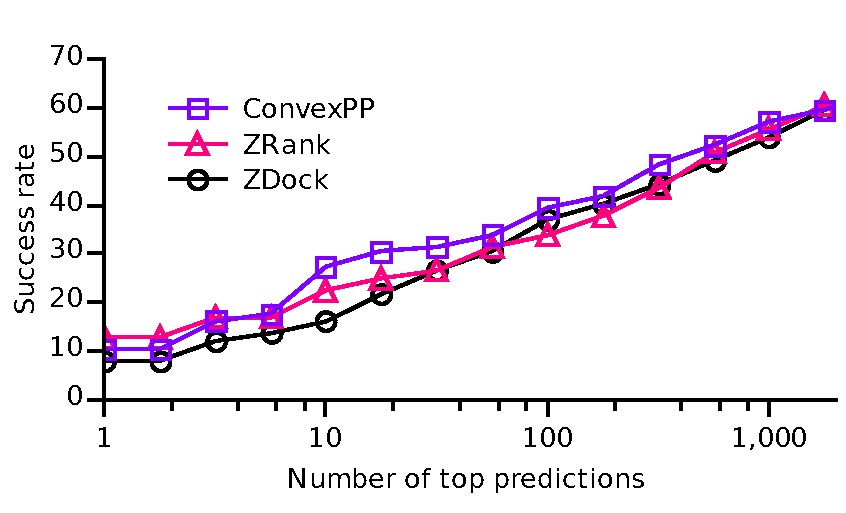
\includegraphics[width=0.5\textwidth]{Scoring/Fig/AllCurvesZDOCKU}
\caption[The success rate on ZDOCK benchmark]{Dependence of the success rate on ZDOCK benchmark on the number of top predictions in consideration for the three methods.}
\label{fig:ROC_ZDOCK} 
\end{center}
\end{figure}

\subsection{Rosetta Benchmark}

Baker, Gray \emph{et al} generated the Rosetta benchmark using 54 complexes of the ZDOCK Benchmark 0.0 \cite{Chen2002} using a flexible docking protocol, 
which is a part of the RosettaDock suite \cite{Gray2003}. 
The first step in the protocol is the 
random translation and rotation of one of the proteins constituting the complex. Afterwards, the side chain is optimized simultaneously with the rigid body displacement. Finally, the full-atom
minimization is done to refine the conformation. For each complex, Baker and Gray generated 1000 decoys following the described protocol. 
The resulting decoys with the corresponding scores assigned by the RosettaDock program can be obtained from \cite{RosettaDecoysLink}. We
calculated the success rate of RosettaDock using the same quality criteria as in Critical Assessment of PRediction of Interactions \cite{Mendez2003,Mendez2005,Janin2009}. 
The Rosetta benchmark contains 5 complexes homologous to the ones present in the training set. Therefore we
trained our scoring function using training sets with and without these homologs (Table S2). 
Table \ref{RosettaTable} compares the results of RosettaDock\cite{Gray2003}, ITScore-PP\cite{Huang2008} and our ConvexPP scoring functions. 

\newpage

\begin{longtable}{c c c c c c|c c c c c|c c c c c}
& 
\multicolumn{5}{c}{RosettaDock} &
\multicolumn{5}{c}{ITScore-PP} &
\multicolumn{5}{c}{ConvexPP} \\
\hline
\begin{sideways}{Complex}\end{sideways}&\begin{sideways}{Quality}\end{sideways}&\begin{sideways}{Rank}\end{sideways}&\begin{sideways}$\mathrm{L_{rmsd}}$\end{sideways}&\begin{sideways}$\mathrm{I_{rmsd}}$\end{sideways}&\begin{sideways}$\mathrm{F_{nat}}$\end{sideways}&\begin{sideways}{Quality}\end{sideways}&\begin{sideways}{Rank}\end{sideways}&\begin{sideways}$\mathrm{L_{rmsd}}$\end{sideways}&\begin{sideways}$\mathrm{I_{rmsd}}$\end{sideways}&\begin{sideways}$\mathrm{F_{nat}}$\end{sideways}&\begin{sideways}{Quality}\end{sideways}&\begin{sideways}{Rank}\end{sideways}&\begin{sideways}$\mathrm{L_{rmsd}}$\end{sideways}&\begin{sideways}$\mathrm{I_{rmsd}}$\end{sideways}&\begin{sideways}$\mathrm{F_{nat}}$\end{sideways}\\ 
 \hline
\textbf{\tiny 1ACB}&\textbf{\tiny 3}&\textbf{\tiny 3}&\textbf{\tiny 9.08}&\textbf{\tiny 3.41}&\textbf{\tiny 0.13}&\textbf{\tiny 3}&\textbf{\tiny 4}&\textbf{\tiny 9.04}&\textbf{\tiny 3.39}&\textbf{\tiny 0.11}&\textbf{\tiny 2}&\textbf{\tiny 1}&\textbf{\tiny 4.31}&\textbf{\tiny 1.13}&\textbf{\tiny 0.78}\\ 
 {\tiny 1A0O}&{\tiny 2}&{\tiny 1}&{\tiny 10.29}&{\tiny 4.18}&{\tiny 0.57}&{\tiny 2}&{\tiny 1}&{\tiny 10.29}&{\tiny 4.18}&{\tiny 0.57}&{\tiny 3}&{\tiny 1}&{\tiny 11.33}&{\tiny 5.79}&{\tiny 0.35}\\ 
 {\tiny 1AHW}&{\tiny 2}&{\tiny 1}&{\tiny 6.41}&{\tiny 2.37}&{\tiny 0.51}&{\tiny 3}&{\tiny 4}&{\tiny 6.46}&{\tiny 3.00}&{\tiny 0.49}&{\tiny 2}&{\tiny 1}&{\tiny 4.82}&{\tiny 2.31}&{\tiny 0.44}\\ 
 {\tiny 1ATN}&{\tiny 3}&{\tiny 1}&{\tiny 5.83}&{\tiny 2.79}&{\tiny 0.49}&{\tiny 3}&{\tiny 1}&{\tiny 9.49}&{\tiny 4.70}&{\tiny 0.38}&{\tiny 1}&{\tiny 1}&{\tiny 2.34}&{\tiny 0.71}&{\tiny 0.77}\\ 
 \textbf{\tiny 1AVW}&\textbf{\tiny 2}&\textbf{\tiny 1}&\textbf{\tiny 6.02}&\textbf{\tiny 2.09}&\textbf{\tiny 0.67}&\textbf{\tiny 2}&\textbf{\tiny 1}&\textbf{\tiny 5.07}&\textbf{\tiny 1.81}&\textbf{\tiny 0.71}&\textbf{\tiny 2}&\textbf{\tiny 1}&\textbf{\tiny 6.01}&\textbf{\tiny 1.38}&\textbf{\tiny 0.75}\\ 
 {\tiny 1AVZ}&{\tiny 3}&{\tiny 37}&{\tiny 8.08}&{\tiny 4.05}&{\tiny 0.29}&{\tiny 3}&{\tiny 22}&{\tiny 11.47}&{\tiny 5.55}&{\tiny 0.35}&{\tiny 3}&{\tiny 20}&{\tiny 8.41}&{\tiny 4.41}&{\tiny 0.12}\\ 
 {\tiny 1BQL}&{\tiny 1}&{\tiny 1}&{\tiny 1.57}&{\tiny 0.86}&{\tiny 0.64}&{\tiny 1}&{\tiny 5}&{\tiny 1.81}&{\tiny 0.72}&{\tiny 0.65}&{\tiny 1}&{\tiny 1}&{\tiny 1.40}&{\tiny 0.96}&{\tiny 0.89}\\ 
 {\tiny 1BRC}&{\tiny 2}&{\tiny 4}&{\tiny 3.77}&{\tiny 1.21}&{\tiny 0.75}&{\tiny 2}&{\tiny 1}&{\tiny 3.77}&{\tiny 1.21}&{\tiny 0.75}&{\tiny 2}&{\tiny 1}&{\tiny 7.24}&{\tiny 1.62}&{\tiny 0.76}\\ 
 {\tiny 1BRS}&{\tiny 2}&{\tiny 1}&{\tiny 4.78}&{\tiny 1.73}&{\tiny 0.64}&{\tiny 3}&{\tiny 1}&{\tiny 8.68}&{\tiny 4.46}&{\tiny 0.33}&{\tiny 3}&{\tiny 1}&{\tiny 8.70}&{\tiny 3.79}&{\tiny 0.31}\\ 
 {\tiny 1BTH}&{\tiny 3}&{\tiny 4}&{\tiny 18.21}&{\tiny 5.54}&{\tiny 0.30}&{\tiny 3}&{\tiny 2}&{\tiny 5.60}&{\tiny 2.35}&{\tiny 0.42}&{\tiny 3}&{\tiny 1}&{\tiny 5.59}&{\tiny 2.67}&{\tiny 0.44}\\ 
 {\tiny 1BVK}&{\tiny 3}&{\tiny 1}&{\tiny 7.91}&{\tiny 3.93}&{\tiny 0.20}&{\tiny 3}&{\tiny 1}&{\tiny 7.18}&{\tiny 3.54}&{\tiny 0.20}&{\tiny 3}&{\tiny 1}&{\tiny 7.75}&{\tiny 3.45}&{\tiny 0.22}\\ 
 \textbf{\tiny 1CGI}&\textbf{\tiny 2}&\textbf{\tiny 2}&\textbf{\tiny 3.79}&\textbf{\tiny 1.86}&\textbf{\tiny 0.50}&\textbf{\tiny 3}&\textbf{\tiny 8}&\textbf{\tiny 6.01}&\textbf{\tiny 2.37}&\textbf{\tiny 0.42}&\textbf{\tiny 3}&\textbf{\tiny 3}&\textbf{\tiny 6.44}&\textbf{\tiny 2.11}&\textbf{\tiny 0.38}\\ 
 {\tiny 1CHO}&{\tiny 3}&{\tiny 1}&{\tiny 6.31}&{\tiny 2.19}&{\tiny 0.46}&{\tiny 3}&{\tiny 1}&{\tiny 10.32}&{\tiny 3.76}&{\tiny 0.18}&{\tiny 2}&{\tiny 1}&{\tiny 6.35}&{\tiny 1.81}&{\tiny 0.66}\\ 
 {\tiny 1CSE}&{\tiny 2}&{\tiny 6}&{\tiny 10.10}&{\tiny 3.12}&{\tiny 0.56}&{\tiny 2}&{\tiny 1}&{\tiny 8.81}&{\tiny 2.66}&{\tiny 0.71}&{\tiny 3}&{\tiny 1}&{\tiny 7.87}&{\tiny 2.29}&{\tiny 0.40}\\ 
 {\tiny 1DFJ}&{\tiny 2}&{\tiny 1}&{\tiny 5.69}&{\tiny 2.66}&{\tiny 0.59}&{\tiny 2}&{\tiny 1}&{\tiny 5.69}&{\tiny 2.66}&{\tiny 0.59}&{\tiny 2}&{\tiny 1}&{\tiny 5.63}&{\tiny 2.55}&{\tiny 0.67}\\ 
 {\tiny 1DQJ}&{\tiny 3}&{\tiny 1}&{\tiny 6.71}&{\tiny 3.35}&{\tiny 0.31}&{\tiny 3}&{\tiny 5}&{\tiny 5.00}&{\tiny 2.12}&{\tiny 0.34}&{\tiny 3}&{\tiny 1}&{\tiny 14.01}&{\tiny 6.06}&{\tiny 0.38}\\ 
 {\tiny 1EFU}&{\tiny 3}&{\tiny 44}&{\tiny 5.98}&{\tiny 3.78}&{\tiny 0.16}&{\tiny 3}&{\tiny 26}&{\tiny 7.83}&{\tiny 4.21}&{\tiny 0.10}&{\tiny 3}&{\tiny 20}&{\tiny 5.90}&{\tiny 4.65}&{\tiny 0.11}\\ 
 {\tiny 1EO8}&{\tiny 3}&{\tiny 1}&{\tiny 10.73}&{\tiny 5.54}&{\tiny 0.31}&{\tiny 3}&{\tiny 31}&{\tiny 6.12}&{\tiny 3.36}&{\tiny 0.15}&{\tiny 3}&{\tiny 1}&{\tiny 10.90}&{\tiny 3.29}&{\tiny 0.42}\\ 
 {\tiny 1FBI}&{\tiny 2}&{\tiny 1}&{\tiny 2.79}&{\tiny 1.37}&{\tiny 0.54}&{\tiny 2}&{\tiny 1}&{\tiny 3.64}&{\tiny 1.86}&{\tiny 0.51}&{\tiny 3}&{\tiny 1}&{\tiny 11.03}&{\tiny 4.23}&{\tiny 0.36}\\ 
 {\tiny 1FIN}&{\tiny 3}&{\tiny 364}&{\tiny 9.88}&{\tiny 5.38}&{\tiny 0.12}&{\tiny 3}&{\tiny 109}&{\tiny 8.26}&{\tiny 4.19}&{\tiny 0.12}&{\tiny 3}&{\tiny 200}&{\tiny 8.27}&{\tiny 6.06}&{\tiny 0.10}\\ 
 {\tiny 1FQ1}&{\tiny 3}&{\tiny 1}&{\tiny 11.37}&{\tiny 5.43}&{\tiny 0.31}&{\tiny 3}&{\tiny 1}&{\tiny 9.33}&{\tiny 5.09}&{\tiny 0.41}&{\tiny 3}&{\tiny 1}&{\tiny 6.79}&{\tiny 4.02}&{\tiny 0.43}\\ 
 {\tiny 1FSS}&{\tiny 1}&{\tiny 1}&{\tiny 3.07}&{\tiny 0.97}&{\tiny 0.74}&{\tiny 2}&{\tiny 1}&{\tiny 4.46}&{\tiny 1.42}&{\tiny 0.46}&{\tiny 2}&{\tiny 1}&{\tiny 3.89}&{\tiny 1.54}&{\tiny 0.63}\\ 
 {\tiny 1GLA}&{\tiny 2}&{\tiny 4}&{\tiny 5.96}&{\tiny 1.85}&{\tiny 0.65}&{\tiny 3}&{\tiny 7}&{\tiny 11.96}&{\tiny 3.83}&{\tiny 0.35}&{\tiny 2}&{\tiny 1}&{\tiny 6.20}&{\tiny 1.70}&{\tiny 0.84}\\ 
 {\tiny 1GOT}&{\tiny 3}&{\tiny 12}&{\tiny 7.86}&{\tiny 3.95}&{\tiny 0.19}&{\tiny 3}&{\tiny 4}&{\tiny 9.71}&{\tiny 4.26}&{\tiny 0.19}&{\tiny 3}&{\tiny 2}&{\tiny 12.91}&{\tiny 3.21}&{\tiny 0.17}\\ 
 {\tiny 1IAI}&{\tiny 3}&{\tiny 8}&{\tiny 6.60}&{\tiny 3.42}&{\tiny 0.22}&{\tiny 2}&{\tiny 1}&{\tiny 4.18}&{\tiny 1.61}&{\tiny 0.62}&{\tiny 2}&{\tiny 1}&{\tiny 3.82}&{\tiny 1.62}&{\tiny 0.33}\\ 
 {\tiny 1IGC}&{\tiny 1}&{\tiny 1}&{\tiny 2.15}&{\tiny 0.63}&{\tiny 0.85}&{\tiny 1}&{\tiny 1}&{\tiny 2.15}&{\tiny 0.63}&{\tiny 0.85}&{\tiny 1}&{\tiny 1}&{\tiny 1.92}&{\tiny 0.56}&{\tiny 1.00}\\ 
 {\tiny 1JHL}&{\tiny 3}&{\tiny 3}&{\tiny 8.56}&{\tiny 4.51}&{\tiny 0.26}&{\tiny 2}&{\tiny 2}&{\tiny 6.09}&{\tiny 2.66}&{\tiny 0.56}&{\tiny 3}&{\tiny 2}&{\tiny 7.65}&{\tiny 3.94}&{\tiny 0.31}\\ 
 {\tiny 1MAH}&{\tiny 2}&{\tiny 1}&{\tiny 3.72}&{\tiny 1.19}&{\tiny 0.70}&{\tiny 3}&{\tiny 1}&{\tiny 8.66}&{\tiny 2.77}&{\tiny 0.26}&{\tiny 2}&{\tiny 1}&{\tiny 3.71}&{\tiny 1.15}&{\tiny 0.78}\\ 
 {\tiny 1MDA}&{\tiny 3}&{\tiny 1}&{\tiny 8.77}&{\tiny 3.59}&{\tiny 0.19}&{\tiny 3}&{\tiny 1}&{\tiny 9.84}&{\tiny 3.92}&{\tiny 0.26}&{\tiny 2}&{\tiny 2}&{\tiny 6.65}&{\tiny 2.38}&{\tiny 0.52}\\ 
 {\tiny 1MEL}&{\tiny 2}&{\tiny 1}&{\tiny 8.47}&{\tiny 2.62}&{\tiny 0.50}&{\tiny 2}&{\tiny 4}&{\tiny 8.47}&{\tiny 2.62}&{\tiny 0.50}&{\tiny 2}&{\tiny 1}&{\tiny 7.89}&{\tiny 2.84}&{\tiny 0.52}\\ 
 {\tiny 1MLC}&{\tiny 2}&{\tiny 7}&{\tiny 4.91}&{\tiny 1.37}&{\tiny 0.52}&{\tiny 3}&{\tiny 1}&{\tiny 15.36}&{\tiny 3.45}&{\tiny 0.20}&{\tiny 3}&{\tiny 1}&{\tiny 15.41}&{\tiny 3.04}&{\tiny 0.24}\\ 
 {\tiny 1NCA}&{\tiny 2}&{\tiny 1}&{\tiny 3.06}&{\tiny 1.53}&{\tiny 0.61}&{\tiny 1}&{\tiny 1}&{\tiny 1.24}&{\tiny 0.64}&{\tiny 0.75}&{\tiny 2}&{\tiny 1}&{\tiny 7.62}&{\tiny 2.13}&{\tiny 0.66}\\ 
 {\tiny 1NMB}&{\tiny 1}&{\tiny 1}&{\tiny 0.90}&{\tiny 0.44}&{\tiny 0.80}&{\tiny 1}&{\tiny 6}&{\tiny 2.66}&{\tiny 0.76}&{\tiny 0.85}&{\tiny 1}&{\tiny 1}&{\tiny 2.66}&{\tiny 0.57}&{\tiny 1.00}\\ 
 \textbf{\tiny 1PPE}&\textbf{\tiny 1}&\textbf{\tiny 1}&\textbf{\tiny 1.38}&\textbf{\tiny 0.52}&\textbf{\tiny 0.73}&\textbf{\tiny 3}&\textbf{\tiny 1}&\textbf{\tiny 7.42}&\textbf{\tiny 2.39}&\textbf{\tiny 0.28}&\textbf{\tiny 1}&\textbf{\tiny 1}&\textbf{\tiny 1.38}&\textbf{\tiny 0.54}&\textbf{\tiny 0.89}\\ 
 {\tiny 1QFU}&{\tiny 2}&{\tiny 1}&{\tiny 3.02}&{\tiny 1.10}&{\tiny 0.64}&{\tiny 1}&{\tiny 4}&{\tiny 2.93}&{\tiny 1.00}&{\tiny 0.69}&{\tiny 1}&{\tiny 1}&{\tiny 3.89}&{\tiny 0.98}&{\tiny 0.67}\\ 
 {\tiny 1SPB}&{\tiny 1}&{\tiny 1}&{\tiny 1.06}&{\tiny 0.62}&{\tiny 0.68}&{\tiny 1}&{\tiny 1}&{\tiny 1.47}&{\tiny 0.70}&{\tiny 0.69}&{\tiny 1}&{\tiny 1}&{\tiny 1.04}&{\tiny 0.54}&{\tiny 0.82}\\ 
 {\tiny 1STF}&{\tiny 1}&{\tiny 1}&{\tiny 1.91}&{\tiny 0.68}&{\tiny 0.89}&{\tiny 1}&{\tiny 2}&{\tiny 1.57}&{\tiny 0.54}&{\tiny 0.91}&{\tiny 1}&{\tiny 1}&{\tiny 1.57}&{\tiny 0.51}&{\tiny 0.94}\\ 
 {\tiny 1TAB}&{\tiny 2}&{\tiny 1}&{\tiny 4.16}&{\tiny 1.30}&{\tiny 0.74}&{\tiny 2}&{\tiny 1}&{\tiny 4.39}&{\tiny 1.37}&{\tiny 0.76}&{\tiny 2}&{\tiny 1}&{\tiny 4.11}&{\tiny 1.47}&{\tiny 0.68}\\ 
 {\tiny 1TGS}&{\tiny 2}&{\tiny 1}&{\tiny 2.48}&{\tiny 1.44}&{\tiny 0.59}&{\tiny 2}&{\tiny 1}&{\tiny 2.26}&{\tiny 1.38}&{\tiny 0.64}&{\tiny 3}&{\tiny 1}&{\tiny 8.41}&{\tiny 3.55}&{\tiny 0.44}\\ 
 {\tiny 1UDI}&{\tiny 2}&{\tiny 1}&{\tiny 3.35}&{\tiny 1.43}&{\tiny 0.63}&{\tiny 2}&{\tiny 1}&{\tiny 2.08}&{\tiny 1.01}&{\tiny 0.74}&{\tiny 2}&{\tiny 1}&{\tiny 2.08}&{\tiny 1.09}&{\tiny 0.71}\\ 
 {\tiny 1UGH}&{\tiny 1}&{\tiny 1}&{\tiny 1.78}&{\tiny 0.86}&{\tiny 0.67}&{\tiny 2}&{\tiny 1}&{\tiny 4.64}&{\tiny 1.90}&{\tiny 0.46}&{\tiny 2}&{\tiny 1}&{\tiny 4.61}&{\tiny 1.96}&{\tiny 0.60}\\ 
 {\tiny 1WEJ}&{\tiny 3}&{\tiny 15}&{\tiny 9.28}&{\tiny 2.92}&{\tiny 0.44}&{\tiny 2}&{\tiny 2}&{\tiny 6.90}&{\tiny 2.55}&{\tiny 0.62}&{\tiny 3}&{\tiny 1}&{\tiny 9.37}&{\tiny 4.79}&{\tiny 0.23}\\ 
 {\tiny 1WQ1}&{\tiny 3}&{\tiny 1}&{\tiny 5.53}&{\tiny 2.46}&{\tiny 0.34}&{\tiny 2}&{\tiny 1}&{\tiny 3.38}&{\tiny 1.92}&{\tiny 0.39}&{\tiny 2}&{\tiny 2}&{\tiny 3.83}&{\tiny 1.59}&{\tiny 0.58}\\ 
 {\tiny 2BTF}&{\tiny 3}&{\tiny 1}&{\tiny 10.03}&{\tiny 3.23}&{\tiny 0.22}&{\tiny 1}&{\tiny 1}&{\tiny 1.52}&{\tiny 0.60}&{\tiny 0.75}&{\tiny 1}&{\tiny 1}&{\tiny 1.31}&{\tiny 0.60}&{\tiny 0.90}\\ 
 {\tiny 2JEL}&{\tiny 2}&{\tiny 1}&{\tiny 4.82}&{\tiny 2.22}&{\tiny 0.52}&{\tiny 2}&{\tiny 1}&{\tiny 6.55}&{\tiny 1.98}&{\tiny 0.65}&{\tiny 2}&{\tiny 1}&{\tiny 6.42}&{\tiny 1.26}&{\tiny 0.86}\\ 
 {\tiny 2KAI}&{\tiny 1}&{\tiny 2}&{\tiny 2.02}&{\tiny 0.97}&{\tiny 0.67}&{\tiny 2}&{\tiny 2}&{\tiny 2.48}&{\tiny 1.05}&{\tiny 0.70}&{\tiny 1}&{\tiny 8}&{\tiny 2.26}&{\tiny 0.89}&{\tiny 0.88}\\ 
 {\tiny 2PCC}&{\tiny 3}&{\tiny 2}&{\tiny 9.19}&{\tiny 3.39}&{\tiny 0.24}&{\tiny 3}&{\tiny 1}&{\tiny 9.38}&{\tiny 3.84}&{\tiny 0.29}&{\tiny 3}&{\tiny 1}&{\tiny 9.40}&{\tiny 4.31}&{\tiny 0.48}\\ 
 {\tiny 2PTC}&{\tiny 1}&{\tiny 4}&{\tiny 0.82}&{\tiny 0.44}&{\tiny 0.80}&{\tiny 2}&{\tiny 4}&{\tiny 5.86}&{\tiny 1.82}&{\tiny 0.70}&{\tiny 2}&{\tiny 1}&{\tiny 5.30}&{\tiny 1.16}&{\tiny 0.74}\\ 
 {\tiny 2SIC}&{\tiny 2}&{\tiny 1}&{\tiny 5.18}&{\tiny 1.53}&{\tiny 0.85}&{\tiny 2}&{\tiny 1}&{\tiny 5.18}&{\tiny 1.53}&{\tiny 0.85}&{\tiny 1}&{\tiny 1}&{\tiny 4.84}&{\tiny 0.96}&{\tiny 0.82}\\ 
 \textbf{\tiny 2SNI}&\textbf{\tiny 2}&\textbf{\tiny 1}&\textbf{\tiny 6.70}&\textbf{\tiny 2.01}&\textbf{\tiny 0.60}&\textbf{\tiny 1}&\textbf{\tiny 1}&\textbf{\tiny 2.88}&\textbf{\tiny 0.99}&\textbf{\tiny 0.73}&\textbf{\tiny 2}&\textbf{\tiny 1}&\textbf{\tiny 7.38}&\textbf{\tiny 2.00}&\textbf{\tiny 0.61}\\ 
 {\tiny 2TEC}&{\tiny 1}&{\tiny 1}&{\tiny 2.46}&{\tiny 0.81}&{\tiny 0.74}&{\tiny 1}&{\tiny 1}&{\tiny 2.59}&{\tiny 0.85}&{\tiny 0.78}&{\tiny 1}&{\tiny 1}&{\tiny 1.97}&{\tiny 0.59}&{\tiny 0.80}\\ 
 {\tiny 2VIR}&{\tiny 3}&{\tiny 1}&{\tiny 7.53}&{\tiny 4.19}&{\tiny 0.26}&{\tiny 2}&{\tiny 2}&{\tiny 5.74}&{\tiny 2.17}&{\tiny 0.70}&{\tiny 2}&{\tiny 1}&{\tiny 5.78}&{\tiny 1.03}&{\tiny 0.67}\\ 
 {\tiny 3HHR}&{\tiny 3}&{\tiny 50}&{\tiny 9.84}&{\tiny 3.95}&{\tiny 0.26}&{\tiny 3}&{\tiny 3}&{\tiny 8.17}&{\tiny 4.03}&{\tiny 0.30}&{\tiny 3}&{\tiny 1}&{\tiny 9.41}&{\tiny 3.47}&{\tiny 0.33}\\ 
 {\tiny 4HTC}&{\tiny 2}&{\tiny 1}&{\tiny 3.81}&{\tiny 1.54}&{\tiny 0.61}&{\tiny 3}&{\tiny 1}&{\tiny 5.95}&{\tiny 2.25}&{\tiny 0.42}&{\tiny 2}&{\tiny 1}&{\tiny 4.04}&{\tiny 1.50}&{\tiny 0.76}\\ 
 \hline
& \multicolumn{5}{c}{\tiny Top1: 66.7\% (36/54)} & \multicolumn{5}{c}{\tiny Top1: 59.3\% (32/54)} & \multicolumn{5}{c}{\tiny Top1: 83.3\% (45/54)}  \\ 
 {\tiny Homologs}& \multicolumn{5}{c}{\tiny Top1 and quality 1: 16.7\% (9/54)} & \multicolumn{5}{c}{\tiny Top1 and quality 1: 11.1\% (6/54)} & \multicolumn{5}{c}{\tiny Top1 and quality 1: 20.4\% (11/54)}  \\ 
 {\tiny included}& \multicolumn{5}{c}{\tiny Top1 and quality 1 or 2: 48.1\% (26/54)} & \multicolumn{5}{c}{\tiny Top1 and quality 1 or 2: 38.9\% (21/54)} & \multicolumn{5}{c}{\tiny Top1 and quality 1 or 2: 57.4\% (31/54)}  \\ 
 & \multicolumn{5}{c}{\tiny Top10 and quality 1 or 2: 61.1\% (33/54)} & \multicolumn{5}{c}{\tiny Top10 and quality 1 or 2: 57.4\% (31/54)} & \multicolumn{5}{c}{\tiny Top10 and quality 1 or 2: 63.0\% (34/54)}  \\ 
 \hline
& \multicolumn{5}{c}{} & \multicolumn{5}{c}{} & \multicolumn{5}{c}{\tiny Top1: 81.5\% (44/54)} \\ 
{\tiny Homologs}& \multicolumn{5}{c}{} & \multicolumn{5}{c}{} & \multicolumn{5}{c}{\tiny Top1 and quality 1: 16.7\% (9/54)}  \\ 
{\tiny excluded}& \multicolumn{5}{c}{} & \multicolumn{5}{c}{} & \multicolumn{5}{c}{\tiny Top1 and quality 1 or 2: 55.6\% (30/54)}  \\ 
 & \multicolumn{5}{c}{} & \multicolumn{5}{c}{} & \multicolumn{5}{c}{\tiny Top10 and quality 1 or 2: 61.1\% (33/54)}  \\
\caption[Rosetta unbound benchmark results]{Rosetta unbound benchmark results. Proteins homologous to the ones in the training set are shown with the bold font.}
\label{RosettaTable} 
 \end{longtable}

Table \ref{RosettaTable} shows that our potentials significantly improve Top1 prediction rate over ITScore-PP and RosettaDock scoring functions while also outperforming them according to the other criteria 
(Top1 and quality 1 \emph{etc.}). We computed the percentage of the structures for which the first acceptable prediction was ranked within the top predictions for each complex and plotted it on 
Fig. \ref{fig:ROC_ROSETTA}. According to the plot our scoring function outputs the plausible structure (quality $\geq$3) for more complexes than ITScore-PP and RosettaDock.
Unlike the results on the ZDock benchmark, the results on the Rosetta unbound benchmark slightly decrease when we remove 
homologous complexes from the training set. Among the prediction quality criteria it is the number of predicted
high quality structures that changed the most. On the other hand Top1 prediction rate stayed almost the same. This observation signalizes that the number of predicted high-quality structures is
amenable to overfitting. Therefore unlike the Top1 criterion, it can not serve as a reliable measure of a scoring function predictive power.
Table \ref{RosettaTableC} shows the per-complex comparison of two scoring functions trained with and without homologs.

\begin{figure}[H]
\begin{center}
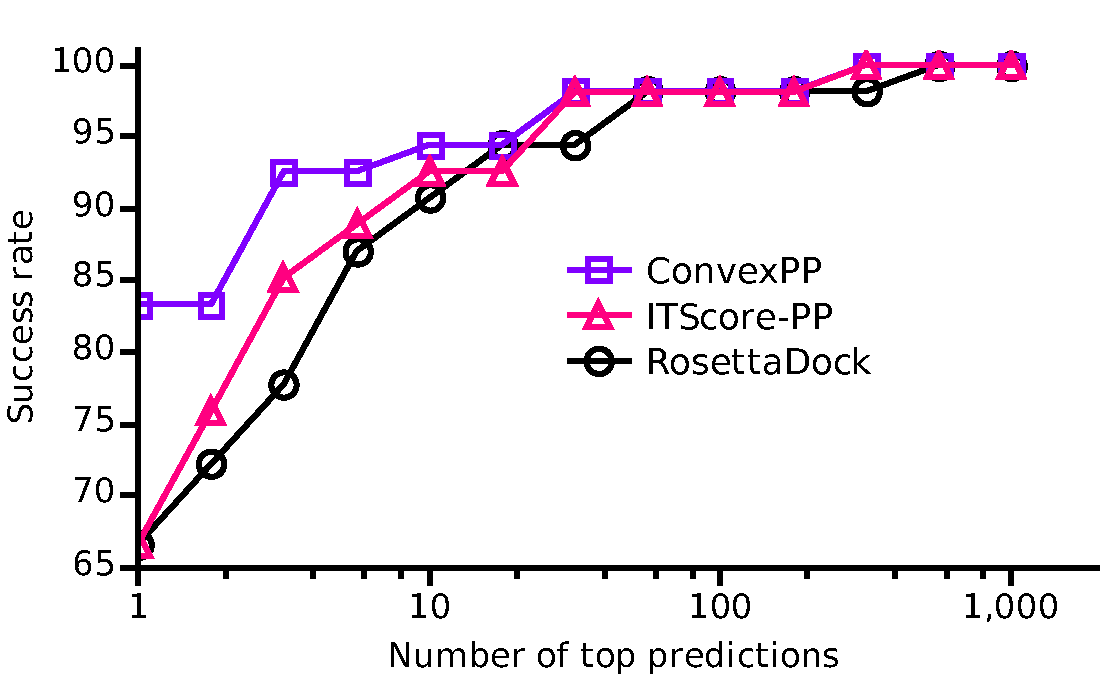
\includegraphics[width=0.5\textwidth]{Scoring/Fig/RosettaU_ROC_Q123All}
\caption[the success rate on Rosetta benchmark]{The percentage of the structures with plausible predictions (quality higher than 3) that are ranked within a certain number of top predictions. 
The data for ITScore-PP was taken from original publication \cite{Huang2008}. Scoring data for RosettaDock was taken from \cite{RosettaDecoysLink}.}
\label{fig:ROC_ROSETTA} 
\end{center}
\end{figure}

\subsection{Water interaction potentials prediction for CAPRI T47 target}

We used the scaled Legendre polynomials as the basis to obtain the potentials for water oxygen interactions. 
Obtained solvation scoring functions for three atom types (aromatic carbon, carboxyl oxygen, and charged nitrogen) are shown in Figure \ref{fig:WaterPotentials}. 
There, one can clearly see the difference between hydrophobic and hydrophilic interactions. Another property of our solvation scoring functions is a same 
peculiarity at short distances as in the other potentials.
Precisely, as there is no training data for distances from 0 to about 2 \AA, all obtained scoring functions are close to zero in this range. 
Therefore, if one would like to use these function for minimization, one might need to adjust them at short distances with some additional information.

\begin{figure}
\begin{center}
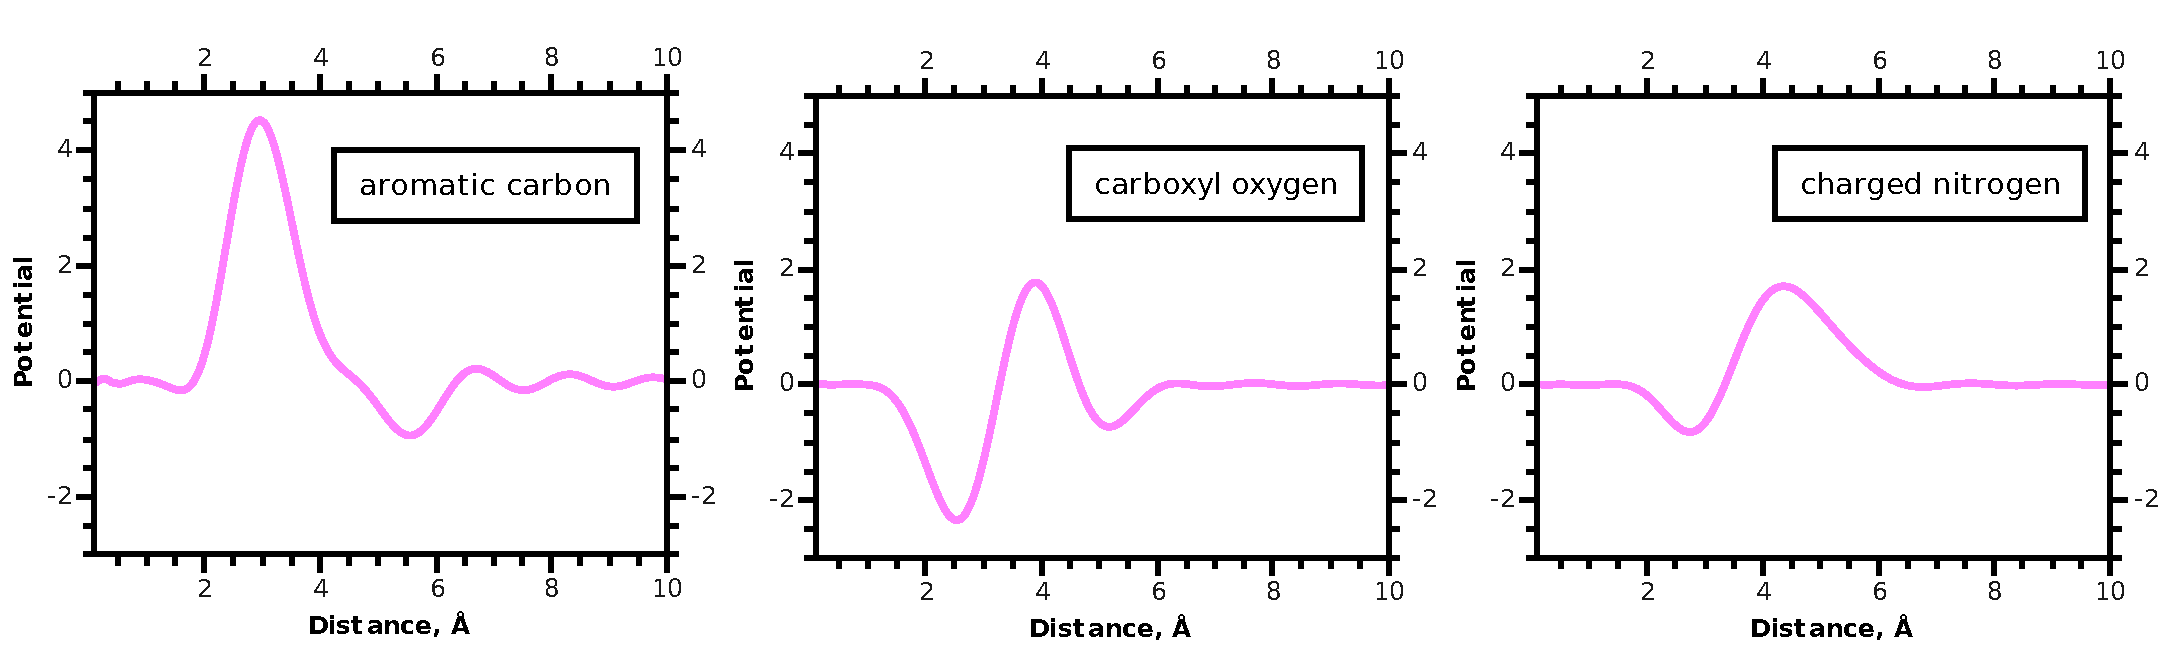
\includegraphics[width=1\textwidth]{Scoring/Fig/3plots_01.pdf}
\caption[Knowledge-based solvation scoring functions]{Knowledge-based solvation scoring functions  $U^{k}(r)$ between the oxygen of a water molecule and 
protein atoms as a function of the separation distance. Left: water -- aromatic carbon scoring function is plotted. 
Middle: water -- carboxyl oxygen (like in aspartic and glutamic acids) scoring function is plotted. Right: water -- charged nitrogen (like in lysins) scoring function is plotted.}
\label{fig:WaterPotentials} 
\end{center}
\end{figure}

The Critical Assessment of Predicted Interaction (CAPRI) \cite{Mendez2003,Mendez2005,Janin2009} is the community-wide competition in prediction of protein-protein complexes. To 
validate our poteintials for water prediction we took part in predicting the structure of the target 47 \cite{lensink2014blind}. The participants were asked to predict the interface of the 
two proteins: DNase domain of colicin E2 and IM2 immunity protein. After docking prediction were performed groups, taking part in this event were invited to predict 
the positions of the water molecules near the interaction interface of the two proteins. Figure \ref{fig:T47XrayStructure} shows the crystall structure of this complex that was
published after the 23rd round of CAPRI ended.

\begin{figure}[H]
\begin{center}
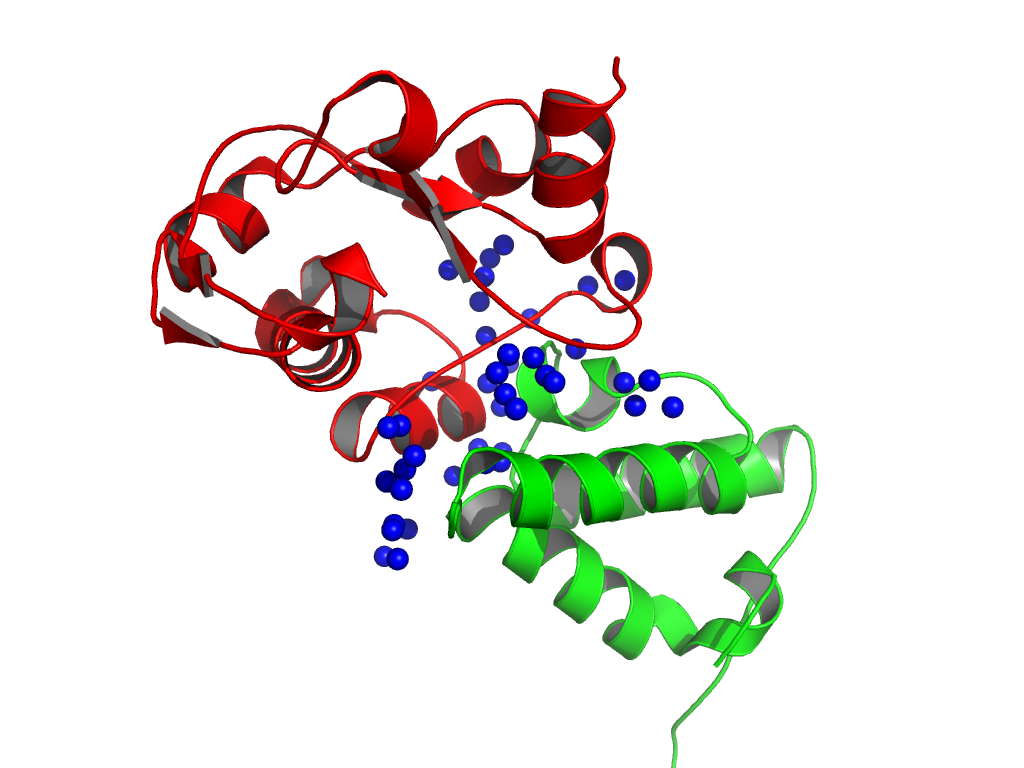
\includegraphics[width=0.5\textwidth]{Scoring/Fig/T47Water.png}
\caption[The crystallographic X-Ray structure of DNase domain of colicin E2 and IM2 immunity protein]{
The crystallographic X-Ray structure of DNase domain of colicin E2 and IM2 immunity protein (PDB code 3U43). IM2 imunity protein is show in green and DNAse domain in red.
Blue spheres denote the positions of interfacial water oxygens. The interfacial water molecule is the one within 3.5\AA~ of both receptor and ligand.}
\label{fig:T47XrayStructure} 
\end{center}
\end{figure}

Each contestant was required to submit 10 models that incuded predicted complex and water molecules. We obtained each model as follows. 
First, we constructed a protein-protein complex by homology using Modeller \cite{eswar2006comparative}. 
Then, we refined the protein-protein interface using our protein-protein docking potentials. 
Finally, we immersed the complex into the water box and minimized the value of the score, obtained by the summation over all interactions between water pseudo-atoms and other atom types,
with respect to the positions of water oxygens.

The criteria  of model quality was based on definition of water-mediated contacts between ligand and receptor. A residue of receptor and a residue of ligand were assumed to
have water-mediated contact when one of their heavy atoms were closer than 3.5\AA~ to the same water oxygen. The quantity $f^{wmc}(nat)$ was computed as the fraction of 
native water-mediated contacts, predicted by the model. Additionally the organizers of the competition computed number of native and model interface water molecules and
number of clashes in each model. The two water molecules assumed to clash if the distance between their oxygen atoms is less than $2.5$\AA. All models were then checked 
for the number of clashes and those where the number of clashing molecules exceeded the number of native interface water molecules were rejected. Other models were
ranked according to the criteria in the Table \ref{Table: waterModelCriteria}.

\begin {table}[H]
 \begin{center}
 \begin{tabular}{ c | c | c  c  c}
  0 & Bad & 0 $\leq$ & $f^{wmc}(nat)$ & $<$ 0.1\\
  + & Fair & 0.1 $\leq$ & $f^{wmc}(nat)$ & $<$ 0.3\\
  2+ & Good & 0.3 $\leq$ & $f^{wmc}(nat)$ & $<$ 0.5\\
  3+ & Excelent & 0.5 $\leq$ & $f^{wmc}(nat)$ & $<$ 0.8\\
  4+ & Bad & 0.8 $\leq$ & $f^{wmc}(nat)$ & $\leq$ 1.0\\
  \end{tabular}
  \caption{Classification of model quality according to the fraction of predicted water-mediated contacts.}
  \label{Table: waterModelCriteria}
  \end{center}
\end{table}

Among the models that we submitted 9 were of good and one of fair quality according to the criterium described above. Overall our approach was ranked 4th 
among others competing techniques. The group ranked first (Nakamura \emph{et all}) and the group ranked third (Zou \emph{et all}) were using the 
water molecules that were derived from the interfaces of the homologs as the initial positions of their predictions. Afterwards they optimized the positions
of water molecules using the AMBER forcefield. The second-ranked group led by Zacharias used \emph{ab-initio} water prediction technique. They combined energy-like
scoring functions with the well-established forcefield (AMBER), energy minimization and short molecular dynamics runs to generate the final predictions.
It is worth to note that our method generated almost no false-positive predictions compared to other competing approaches (\cite{lensink2014blind}, SI).


\subsection{Discussion}
\subsubsection{Short Distances}

\begin{figure}[H]
\begin{center}
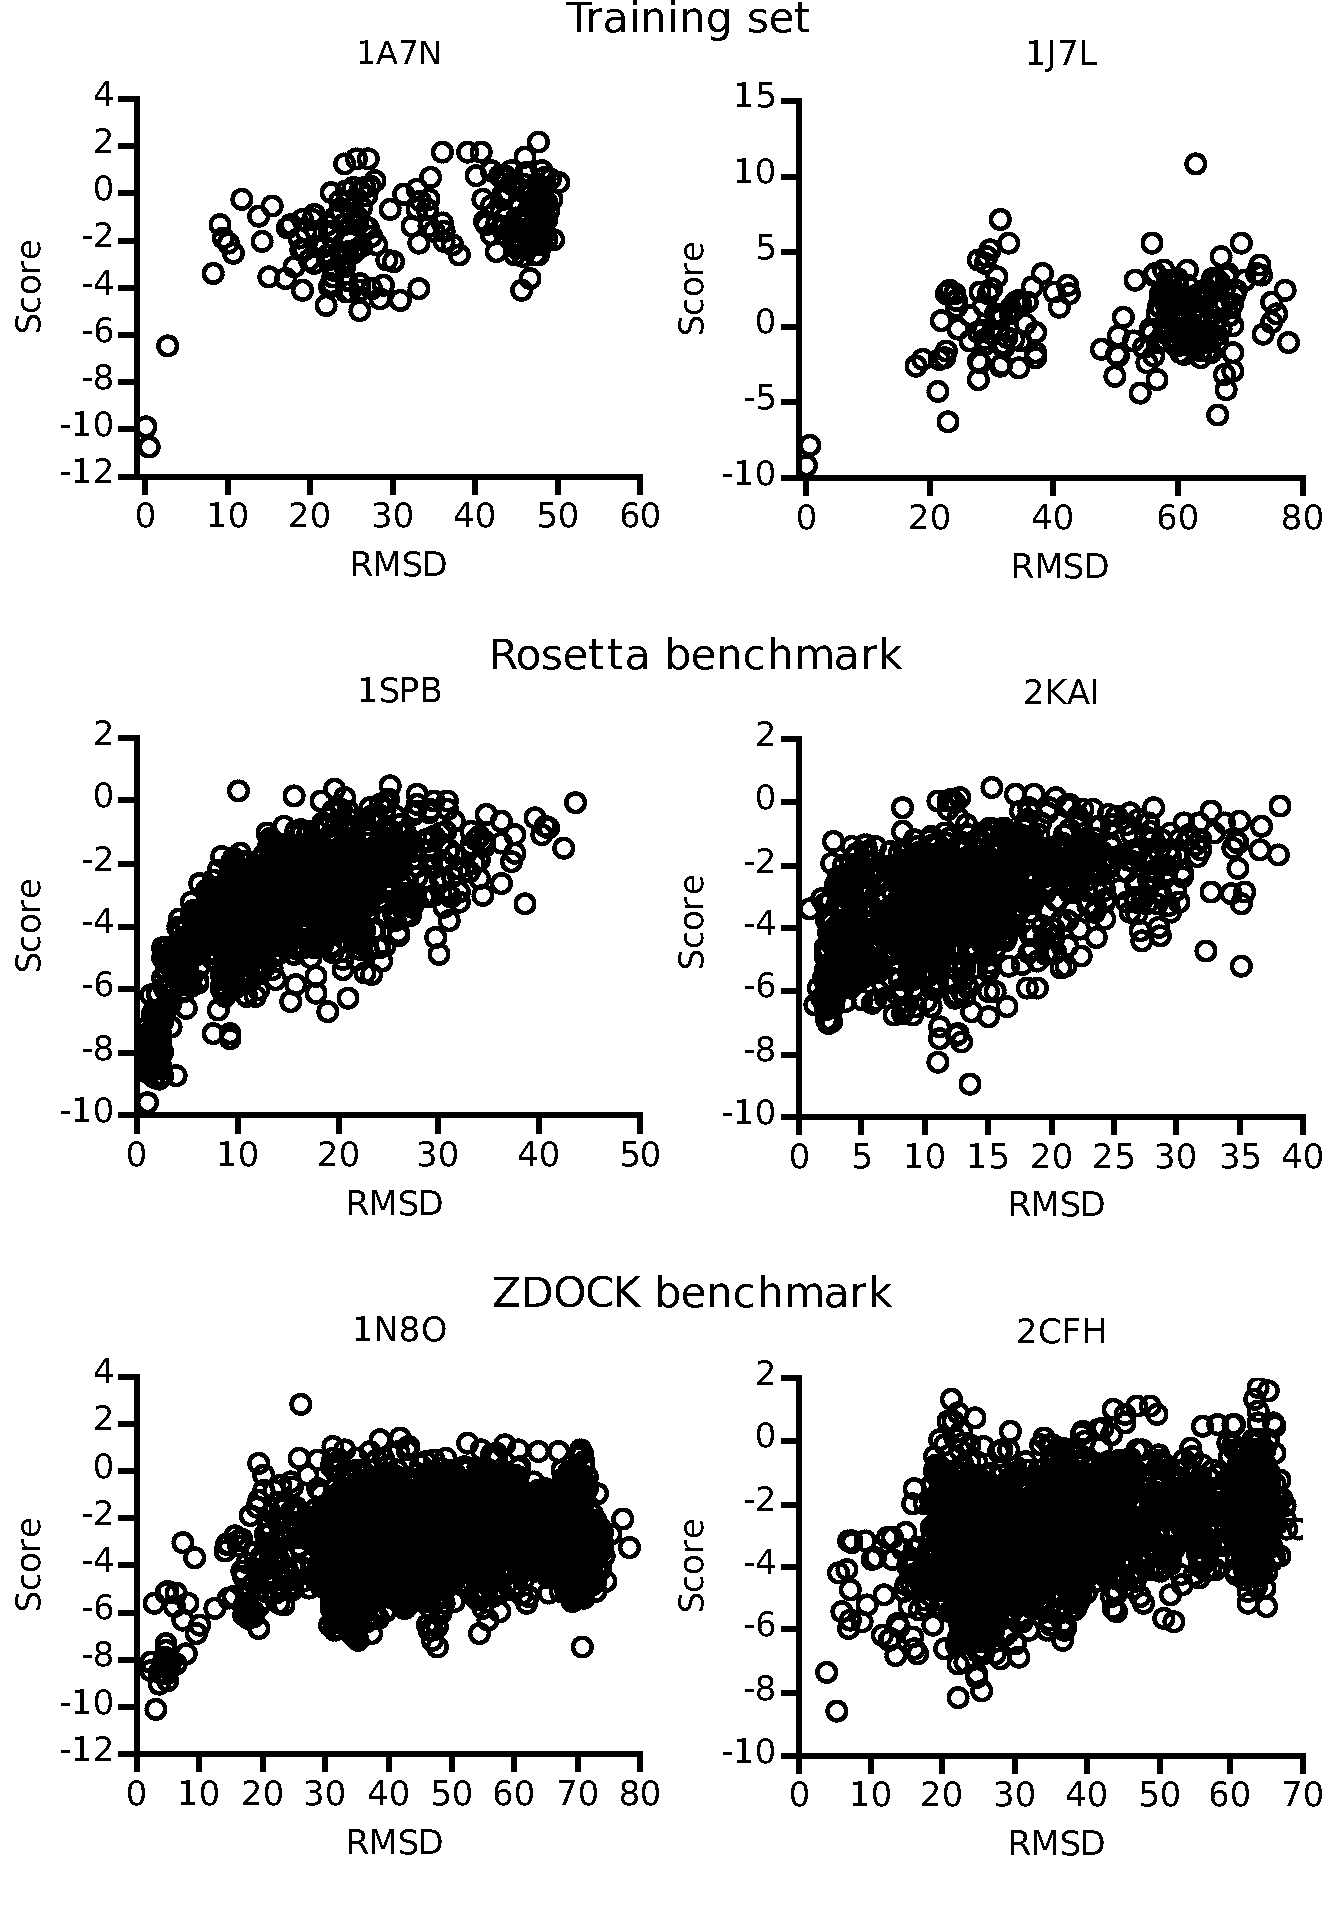
\includegraphics[scale=0.3]{Scoring/Fig/AllFunnels}
\caption[The plots of the ConvexPP versus the lRMSD for the decoy structures]{The plots of the ConvexPP versus the lRMSD for the decoy structures
from the training set (1A7N, 1J7L), Rosetta benchmark (1SPB, 2KAI) and ZDOCK benchmark(1N8O, 2CHF). 
On the left we show the plots that exhibit funnel-like behaviour near the frame origin. On the right side the plots
without obvious funnels are shown.
}
\label{fig:funnels} 
\end{center}
\end{figure}

%Figure \ref{fig:potentials} clearly shows that the scoring potentials obtained have no clear physical interpretation \red{[at short distances!!!]}. 
The key property of a scoring function is the existence of the correlation between the score of a structure and its similarity to the corresponding native structure. 
%Conventionally, the RMSD of one complex subunit (ligand) with the other (receptor) aligned is called lRMSD and is taken as the measure of similarity of two structures 
Conventionally, the lRMSD is taken as the measure of similarity of the decoys to the native structure. 
lRMSD is the ligand (the smaller protein in a complex) root mean square deviation of $C_\alpha$ atoms of a decoy relative to the native complex structure when 
receptors (the larger proteins in the complexes) are superposed.
To verify that our potentials indeed correlate with the similarity to the native structures, we plotted the ConvexPP score of 
each decoy versus the lRMSD for all decoys from the ZDOCK and Rosetta benchmarks. 
%
Figure \ref{fig:funnels} shows some typical plots for the complexes from the training set and the two benchmarks.
%
Typically, in the training set we see a wide separation between native and non-native structures. This happens because decoys in the training set have only a 
few {\em near-native} structures with lRMSD$<$10\AA. On the contrary, about 28\% of the Rosetta decoys are the near-native structures. The 
ZDOCK benchmark has few near-native decoys compared to Rosetta, only 1.5\% of the decoys have the near-native conformations.

For the decoys from the ZDOCK and Rosetta benchmarks, we computed the Pearson correlation between lRMSD and the score using near-native decoys with lRMSD$<$10\AA. In this calculation, 
we considered only the structures that have at least 50 such decoys. All 54 complexes from the Rosetta benchmark
fulfilled this criterion whereas only 24 complexes from the ZDock benchmark had more than 50 near-native decoys.
The average Pearson correlation for the Rosetta benchmark is $0.31$ whereas for the ZDock benchmark it is approximately $0.21$.
We investigated the reason of this discrepancy by looking at the atom-pairs distance distributions of the decoys from the training set, the ZDock and Rosetta benchmarks.
For our analysis, we used decoys of the three common structures from these sets, PDB codes 1PPE, 1CGI, 1ACB. For these decoys, we computed the average total number of 
atom pairs at a certain distance using Eq. \ref{eq:number_density}.
Then, we normalized these distributions on a reference number of pairs  ${\alpha r^3}$. We tuned coefficient $\alpha$ in such a way to make each plot approach the value 1.0 
when the distance approaches 12.0\AA.
%where we tuned the coefficient $\alpha$  to minimize 
%the function $ \left| \sum_{8\AA<r<10\AA} n(r,\alpha) - 1 \right| $ \red{[not very clear what is this function... Can we write without $n(r,\alpha)$?]} for each distribution individually.
%
Figure \ref{fig:histAll} plots normalized atom-pairs distance distributions for the three above-mentioned complexes. From this figure we see that 
the distance distributions for the Rosetta benchmark are much closer to the native distributions compared to the ZDOCK and training set distributions. 
We can also see that the Hex docking program \cite{ritchie2000protein}, which we used for the generation of the training set, produces fewer short-distance atom contacts compared to ZDOCK. 
Since Rosetta decoys were additionally minimized using the Rosetta scoring function, they do not have short-distance atom contacts and generally their distance 
distributions resemble the native statistics.
%the average distribution among decoys from Rosetta benchmark is much closer to the distribution computed
%from the native structure, than the distributions of Training set and
%ZDock decoy set. 
%
%The support vector machines are mostly applicable in the vicinity of the native pair distance distribution \red{[Brrrrrrr. Has no sense, I'll write it]}. 
%That ca be one of the reasons why the correlation for ZDock benchmark is far less than for the Rosetta.
%
Native structures neither have statistics at short distances. Therefore, reconstructed potentials in the vicinity of zero are not reliable and can not provide 
fair scores for e.g. decoys generated with ZDOCK, since these decoys have many short-distance contacts. 
%
Ideally, one needs to additionally penalize short-distance contacts using, e.g., empirical scores that cannot be obtained with statistics from the native structures. 
However, in this study we do not attempt to provide such additional penalization and only focus on the potentials directly obtained from the training set of the protein structures.

\begin{figure}[H]
\begin{center}
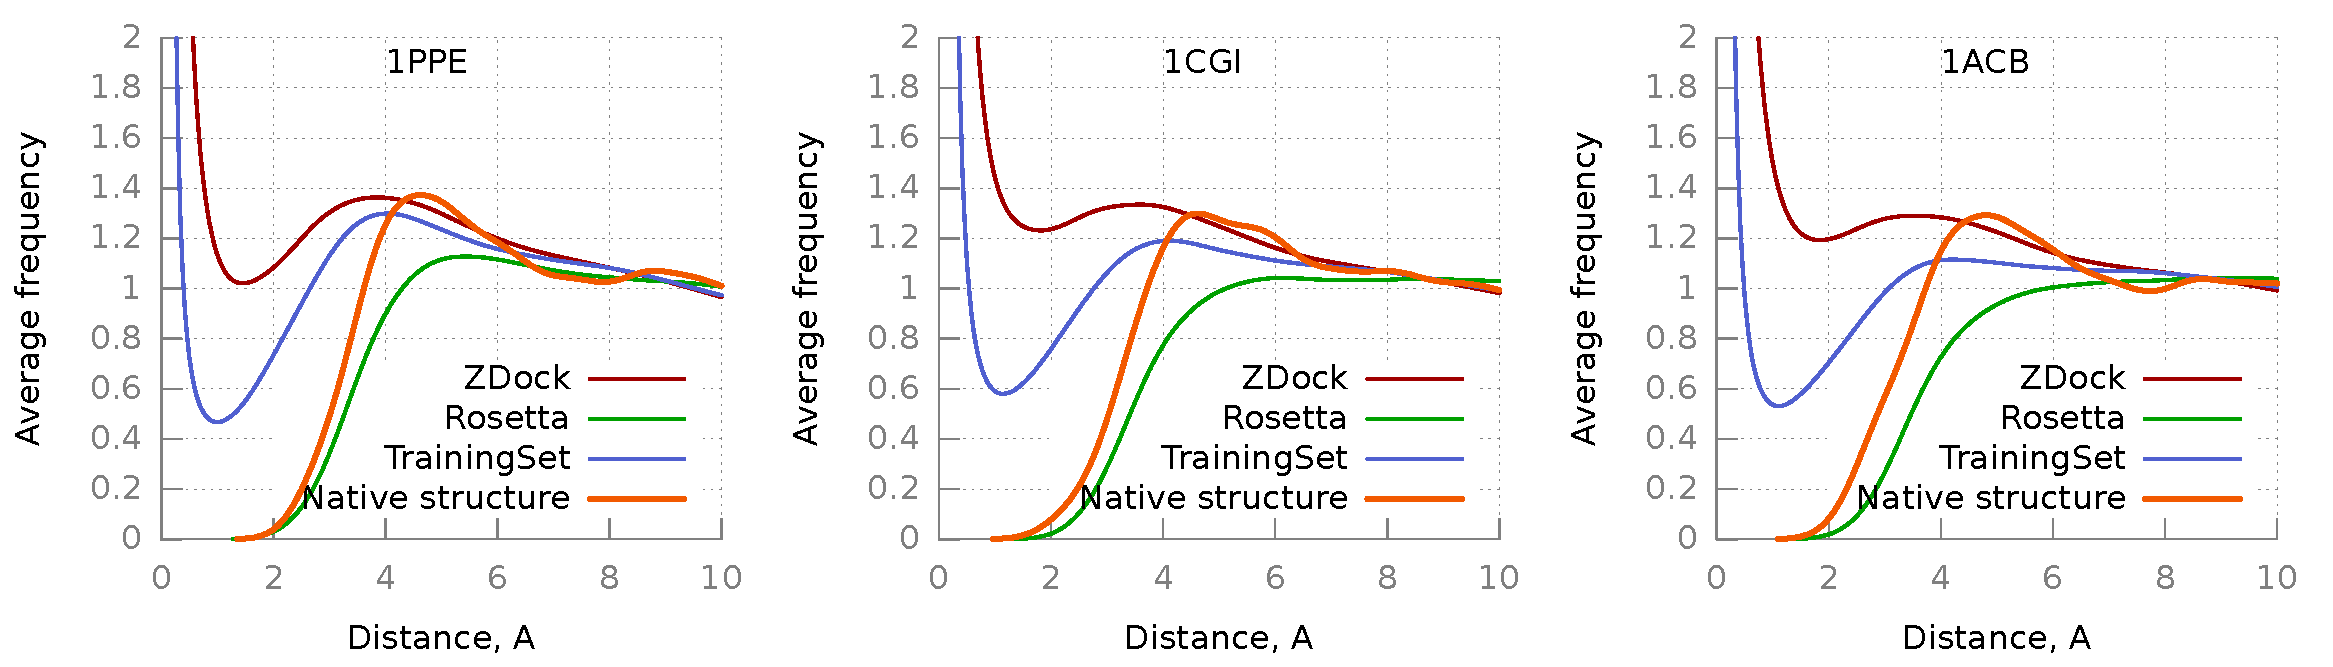
\includegraphics[scale=0.3]{Scoring/Fig/histAllTogether}
\caption[The normalized atom-pairs distance distributions for three complexes 1PPE, 1CGI, and 1ACB]{
The normalized atom-pairs distance distributions for three complexes 1PPE, 1CGI, and 1ACB. For each complex, four plots are shown:
average ZDOCK distribution, average Rosetta distribution, average training set  distribution and the native distribution.
The average is taken over all decoys from the two benchmarks and the training set. 
}
\label{fig:histAll} 
\end{center}
\end{figure}

\subsubsection{Filtering}

%One of the properties of our algorithm that distinguishes it from the others is that our potentials are inherently smooth.
Some knowledge-based potentials are smoothed with a smoothing filter {\em a posteriori}.
%smoothing filter is applied after the potentials are obtained. 
For example, Mitchel et al. \cite{mitchell1999bleep} and Huang et al. \cite{Huang2008} used a ``1:2:4:2:1'' filter, 
DOPE potential is smoothed using cubic polynomials \cite{shen2009statistical}, etc. 
%
On the contrary, our method introduces an assumption about interaction pair distance uncertainty {\em a priory}. 
More specifically, we collect statistics using gaussian events of a variance $\sigma$ (Eq. \ref{eq:number_density}). We determine the value of the variance  
from the afore-mentioned cross-validation procedure.
% by maximising the number of guessed structures in the test set. 
Then, according to Eqs. \ref{eq:scoring_1}--\ref{eq:scoring_2}, ConvexPP scoring function is smooth by construction. 
In other words, we do not need to apply a smoothing 
filter to the obtained potentials, since we introduce the uncertainty when we collect statistics.

Another parameter that  indirectly influences the smoothness of the resulting potential is the regularization parameter $C$ (\ref{eq:regularizationParameter}).
According to Eq. \ref{eq:scoringVector}, the scoring vector $\mathbf{w}$, from which the scoring potentials are derived, is a weighted sum of the support structure vectors $\mathbf{x}_{ij}$.
The more support structure vectors are in the sum, the more regular the scoring vector $\mathbf{w}$ will be. 
%
On the other hand, this number equals to the number of non-zero
Lagrange multipliers $\lambda_{ij}$ (Eq. \ref{eq:scoringVector}) ,  which is uniquely defined by the value of the regularization parameter $C$ \cite{pontil1998properties}. 
Decreasing $C$ results in the increase of the number of non-zero $\lambda_{ij}$ therefore resulting in smoother scoring potentials. 
We also determine the value of this parameter by the cross-validation procedure.

The consistent determination of the two parameters $\sigma$ and $C$  allows us to obtain smooth potentials (Eq. \ref{eq:scoring_2}) 
directly as the solution of the optimization problem (Eq. \ref{eq:svmSoftMargin}).

\subsubsection{Uniqueness of the solution and the reference state}

The concept of the statistical knowledge-based potentials is based on the definition of two states: the observed state and the reference state \cite{Tanaka1976, miyazawa1985estimation, sippl1990calculation}.
The observed state is usually the state when a single protein or a complex has the native conformation. It can be derived from the crystal structures.
Reference state was introduced as an atom pair distance distribution when the interactions between the atom pairs are absent. The knowledge-based potential is then expressed in terms of these two states as:
$$u_{ij}(r) = -RT\ln \left( \frac{N^{obs}_{ij}(r)/N^{obs}_{ij}}{N^{ref}_{ij}(r)/N^{ref}_{ij}} \right), $$ where $N^{ref}_{ij}(r)$ and $N^{obs}_{ij}(r)$ are the numbers of atomic pairs $i,j$ at a distance
$r$ in the reference and observed states, correspondingly, and numbers $N^{ref}_{ij}$ and $N^{obs}_{ij}$ are the total numbers of pairs $i,j$ in these states.
%
Some widely used approaches to derive the reference state for protein folding are the ideal-gas approximation \cite{zhou2002distance}, 
the shuffling of atoms \cite{rykunov2007effects}, a random-walk chain \cite{zhang2010novel}, etc. For protein docking 
Chuang \emph{et al.} used decoys as the reference state \cite{chuang2008dars}, Bernard and Samudrala took the average over the atomic pairs and a cumulative distribution function for all pairs 
as two reference states \cite{bernard2009generalized}, etc. The very wide variety of approaches to derive the reference state has its roots in the loose definition and the complexity of the problem. 
%Therefore one of the advantages of our algorithm over the statistical knowledge-based potentials is that we avoid the computation of the reference state.

%
Recently, the new algorithms that avoid the reference state calculation appeared. We should mention the iterative scheme used by Huang et al.\cite{Huang2008} and the neural network classifier by 
Chae et al. \cite{chae2010predicting}.
These algorithms indeed avoid the definition of the reference state. However, they do not guarantee the uniqueness of their solution. On the contrary, we showed that our 
algorithm converges to the global minimum of the function (Eq. \ref{eq:svmSoftMargin}). Thus, we avoid dependence on the initial guess of the interaction potential.
%The advantage of our algorithm over the abovementioned is the proven convergence (see lemma \ref{lemma:2}) to the global minimum of the functional \ref{eq:svmSoftMargin}. 
%In case of ITScore by Huang or neural network by Chae one can not be sure that the obtained scoring function is the single one for the given decoy set and the parameters of the algorithm. 